%==============================================================================
\chapter{In silico personalised rat heart contraction models: the role of sarcomere kinetics in diastolic heart failure}\label{cha:chapter4}
%==============================================================================
%
%
%
\begin{remark}{Outline}
    In this chapter, we personalise the $3$D biventricular rat heart contraction mechanics mathematical model to the specific clinical data obtained from a cohort of sham-operated and $6$-weeks-post-surgery aortic banded rats. We specifically fit one representative model for each cohort (control and diseased ones). Models' sensitivities are then characterised. Differences in the parameter space between the two models confirm that impaired cardiac function is linked to altered sarcomere kinetics. 
\end{remark}


%
%
%
\section{Motivation}
% Heart contraction is the result of integrated cellular, tissue and organ function. Biophysical \textit{in silico} cardiac models offer a systematic approach for studying these multi-scale interactions. The computational cost of such models is high, due to their multi-parametric and non-linear nature. This has so far made it difficult to perform model fitting and prevented global sensitivity analysis studies. We propose a machine learning approach based on Gaussian process emulation of model simulations using probabilistic surrogate models, which enables model parameter inference via a Bayesian history matching technique and global sensitivity analysis on whole-organ mechanics. This framework is applied to model healthy and aortic-banded hypertensive rats, a commonly used animal model of heart failure disease. The obtained probabilistic surrogate models accurately predicted the left ventricular pump function ($R^2=0.92$ for ejection fraction). The history matching technique allowed us to fit both the control and diseased virtual bi-ventricular rat heart models to MRI and literature data, with model outputs from the constrained parameter space falling within $2$ STD of the respective experimental values. The global sensitivity analysis identified Troponin C and cross-bridge kinetics as key parameters in determining both systolic and diastolic ventricular function.


\todo{this is Introduction copy-pasted from the paper: adapt it to thesis}

\noindent
With each beat, cardiac myocytes generate tension and relax. Cellular tension is transduced into a coordinated, global whole-heart deformation resulting in an effective, system-level pump function. The integration of cellular, tissue and organ-scale mechanisms is essential for achieving efficient transduction of work into concerted myocardial contraction and relaxation. The break down of this system of integrated mechanisms can give rise to heart failure (HF). 

Cardiac biophysical models provide a useful tool for studying whole-organ contraction \cite{Niederer:2019} by simulation, and can therefore be used to understand how impaired cell level function is linked with impaired organ level activity. Building a virtual representation of the real system requires tuning the cardiac model's properties and boundary conditions to experimental data. Global sensitivity analysis (GSA) studies are also needed to determine the role of cellular, tissue and haemodynamics properties on whole-organ function.

However, the high simulation cost and the multi-scale nature of the cardiac system have limited the formal parameter estimation and sensitivity analysis for this type of model. Different techniques have been employed for global parameter inference on cardiac cell models, including gradient descent \cite{Dokos:2004}, genetic algorithms \cite{Groenendaal:2015}, multivariate regression \cite{Sarkar:2010} and Markov chain Monte Carlo (MCMC) \cite{Johnstone:2016}. Most of these approaches are computationally intensive, and the computation burden is even higher when going from single to multiple scales.

Surrogate models (or \textit{emulators}) can be used to replace the computationally expensive real model with a statistical representation of it, allowing rapid predictions of the model's output. Using emulators we can thus perform the high number of model evaluations required to estimate global sensitivities. In this study, we use Gaussian process emulators (GPEs), which provide confidence bounds on predictions and can therefore be used for Bayesian history matching (HM). Previously employed for fitting models of galaxy formation \cite{Vernon:2010}, infectious disease transmission \cite{Andrianakis:2015} and, more recently, human atrial cell~\cite{Coveney:2018}, HM has shown to be a valuable tool for global parameter inference.

To demonstrate the capacity of GPE and HM to fit a virtual heart model, we tune model mechanics-related parameters to data from control and left ventricular (LV) hypertrophied rat hearts. LV hypertrophy is induced surgically by constricting the ascending aorta over $4$ to $6$ weeks and represents a common pathway to HF development. Aortic-banded (AB) rats are commonly used as an experimental animal model for HF pathology~\cite{Camacho:2016}.

We also seek to quantitatively characterise the AB rats' impaired LV contractile function. We therefore fit the virtual bi-ventricular rat model to changes in function that we measured or were recorded by others, using HM. Finally, we perform a GSA to understand how uncertainty in cell, tissue and haemodynamics model properties affect LV function.



%
%
%
\section{Rat data}
We used healthy control and diseased rat data from experimental studies conducted by R{\o}e et al. \cite{Roe:2017}. Briefly, \textit{aortic banding} (\acs{AB}) was performed in male Wistar rats ($n=29$), while \textit{sham-operated} (\acs{SHAM}) rats ($n=23$) served as controls. \textit{In vivo} cardiac function was characterised by echocardiography six weeks after surgery. The criterion for inclusion in the AB group was posterior wall thickening ($>1.9$ mm). A cohort of rats ($n=8$, $n=15$ from SHAM, AB groups, respectively) underwent an examination with \textit{magnetic resonance imaging} (\acs{MRI}). Rats in the AB cohort showed a preserved systolic function (ejection fraction and fractional shortening). Concentric LV hypertrophy arose, as an increase in LV mass and wall thickness was observed. Moreover, evidence of reduced peak early diastolic velocity (e’) and increased early mitral inflow velocity / mitral annular early diastolic velocity (E/e’) confirmed an impaired diastolic function in the rats.


%
%
%
\section{Methods}\label{sec:ch4methods}

%
%
%
\subsection{Mesh generation}\label{sec:ch4meshgeneration}
One representative cine MRI scan was obtained for both the SHAM and the AB rat cohorts. Each image set consisted of $47$ equally, $\SI{2.779}{\milli\second}$-spaced time frames. Example apicobasal slices are shown in Figure~\ref{fig:ratrepimag}, while MRI characteristics are reported in Table~\ref{tab:mrichar}.

\begin{figure}[hbt!]
    \myfloatalign
    \subfloat[SHAM]
    {\label{fig:ratrepimag-a}
    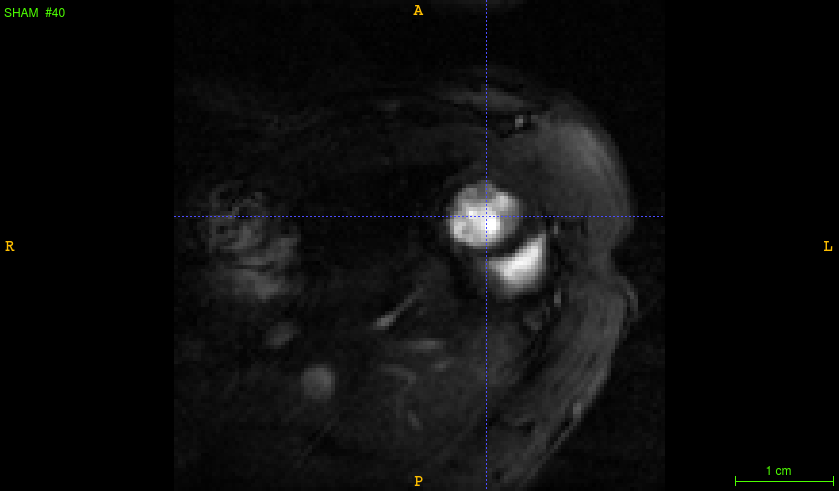
\includegraphics[width=.45\linewidth]{figures/chapter04/sham_image.png}}\quad
    \subfloat[AB]
    {\label{fig:ratrepimag-b}
    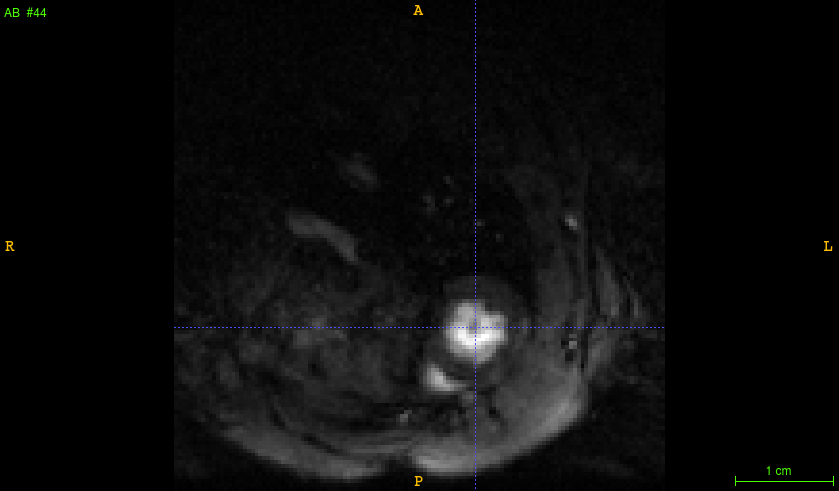
\includegraphics[width=.45\linewidth]{figures/chapter04/ab_image.png}}
    \caption{Rat representative MR Images.}\label{fig:ratrepimag}
\end{figure}

\begin{table}[hbt!]
    \myfloatalign
    \begin{tabularx}{\textwidth}{XXX}
    \toprule
    \tableheadline{Rat} & \multicolumn{2}{c}{\spacedlowsmallcaps{MRI characteristics}} \\
    \midrule   
    & \tableheadline{Size ($\#$voxels)} & \tableheadline{Voxel size ($\SI{}{\cubic\milli\meter}$)} \\
    \cmidrule{2-3}
    SHAM & $128\times 128\times 9$ & $0.39\times 0.39\times 1.5$ \\
    AB   & $128\times 128\times 9$ & $0.39\times 0.39\times 1.5$ \\
    \bottomrule
    \end{tabularx}
    \caption{MRI characteristics.}
    \label{tab:mrichar}
\end{table}

\vspace{0.2cm}
For each rat, we segmented the LV blood pool at each time frame and collected the corresponding volume estimates based on voxels size/count. This allowed to extract LV volume transient for each rat, displayed in Figure~\ref{fig:lvvexptransients}.

\begin{figure}[!ht]
    \myfloatalign
    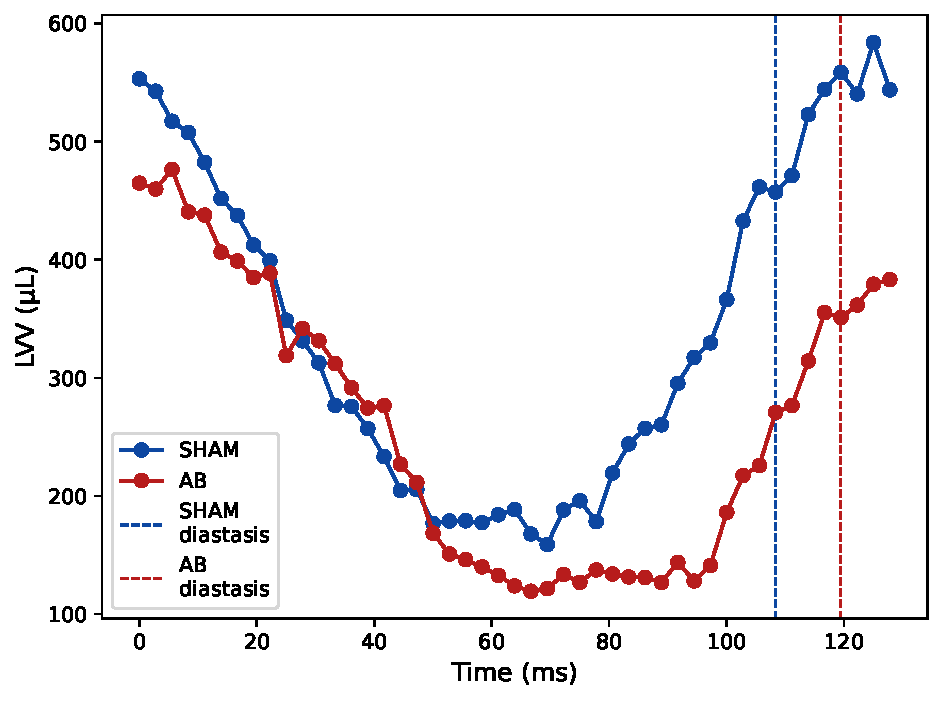
\includegraphics[width=0.8\textwidth]{figures/chapter04/lvv_experimental_transient.pdf}
    \caption{LV volume transients obtained by segmenting the LV blood pool of $47$ consecutive time frames images for the SHAM (blue) and the AB (red) reference rat images. Dashed lines indicate approximately diastasis time during the cardiac cycle.}
    \label{fig:lvvexptransients}
\end{figure}

\vspace{0.2cm}
Time frames were numbered from $1$ to $47$. Frame $\#1$ was assumed to be moment when the heart enters the ejection phase of the cardiac cycle. In order to approximate the stress-free configuration for mechanics simulations, we selected a time frame halfway through diastole which could possibly represent cardiac diastasis (specifically frame $\#40$, $\#44$ for the SHAM, AB rats respectively). We segmented the entire biventricular anatomy at these time frames, comprising three main tags: the LV and RV blood pools and the surrounding myocardium. All the segmentations were performed manually using \texttt{ITK-SNAP} (v.$3.6.0$)~\cite{Yushkevich:2006}. Obtained segmentations are displayed in Figure~\ref{fig:ratrepseg} and estimated volumes are summarised in Table~\ref{tab:segmchar}.

\begin{figure}[ht!]
    \myfloatalign
    \subfloat[SHAM]
    {\label{fig:ratrepseg-a}
    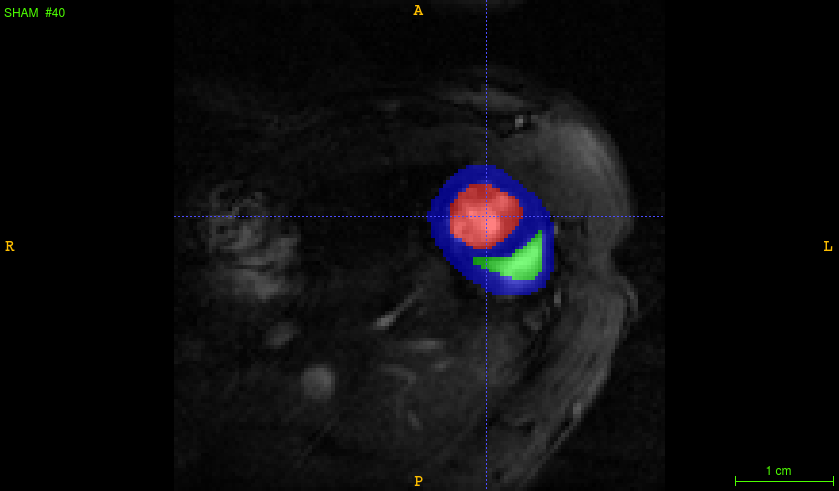
\includegraphics[width=.45\linewidth]{figures/chapter04/sham_segmentation.png}}\quad
    \subfloat[AB]
    {\label{fig:ratrepseg-b}
    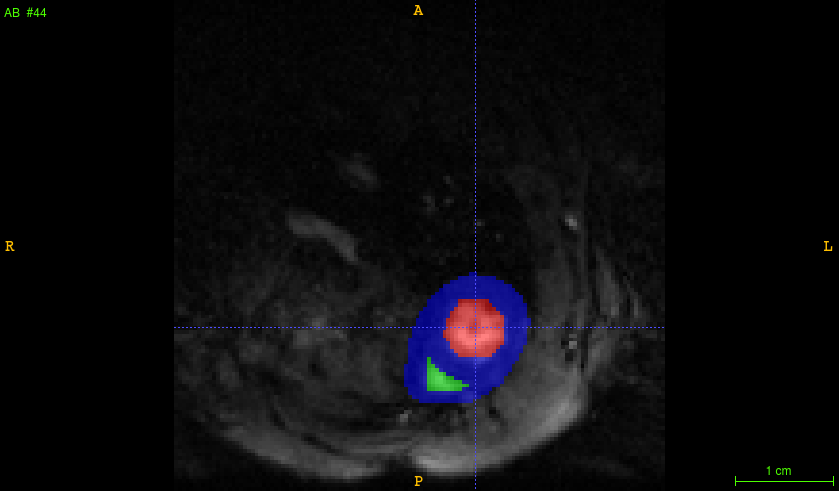
\includegraphics[width=.45\linewidth]{figures/chapter04/ab_segmentation.png}}
    \caption{Rat representative MRI scans segmentations. LV and RV blood pools and myocardium are tagged with respectively red, green and blue colours.}\label{fig:ratrepseg}
\end{figure}

\begin{table}[ht!]
    \myfloatalign
    \begin{tabularx}{\textwidth}{XXXX}
    \toprule
    \tableheadline{Rat} & \multicolumn{3}{c}{\spacedlowsmallcaps{Segmentation characteristics}} \\
    \midrule   
    & \tableheadline{LV ($\SI{}{\cubic\milli\meter}$)} & \tableheadline{RV ($\SI{}{\cubic\milli\meter}$)} & \tableheadline{Myocardium ($\SI{}{\cubic\milli\meter}$)} \\
    \cmidrule{2-4}
    SHAM & $459.14$ & $417.94$ & $1127.93$ \\
    AB   & $357.97$ & $212.17$ & $1181.72$ \\
    \bottomrule
    \end{tabularx}
    \caption{Segmentation tags volume estimates based on voxels size/count.}
    \label{tab:segmchar}
\end{table}

\noindent
Rat meshes with fibres were generated from the representative MRI scans segmentations using the approach described in Section~\ref{sec:ch2anatomy}. We opted for an LoD of $2$ for both the SHAM and the AB mesh generation, as we prioritised stability for mechanics simulations over accuracy. The generated meshes are shown in Figure~\ref{fig:ratrepgeom}.

\begin{figure}[!ht]
    \myfloatalign
    \subfloat[SHAM]
    {\label{fig:ratrepgeom-a}
    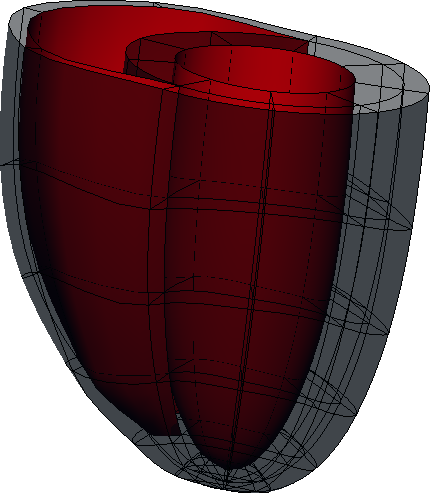
\includegraphics[width=.3\linewidth]{figures/chapter04/sham_mesh.png}}\quad
    \subfloat[AB]
    {\label{fig:ratrepgeom-b}
    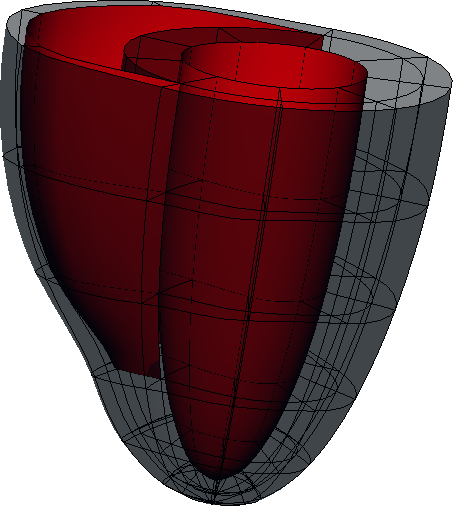
\includegraphics[width=.3\linewidth]{figures/chapter04/ab_mesh.png}}
    \caption{Rat representative cubic Hermite finite element meshes.}
    \label{fig:ratrepgeom}
\end{figure}


%
%
%
\subsection{Ionic model}\label{sec:ch4ionicmodel}
We employed two variants~\cite{Gattoni:2017} of the original ionic model~\cite{Gattoni:2016} the same authors developed in order to describe the control SHAM and the diseased AB rats specific calcium dynamics. The experimental data the authors used to re-fit the original model comes from exactly the same experimental study (\cite{Roe:2017}) which we obtained the MRI scans from. For this reason, we were able have both sham-operated and aortic-banded rat cohorts-specific anatomy and electrophysiology mathematical descriptions at the same time. Simulated action potentials and calcium transients from the two different models are shown in Figure~\ref{fig:shamvsabcaap}.

\begin{figure}[!ht]
    \myfloatalign
    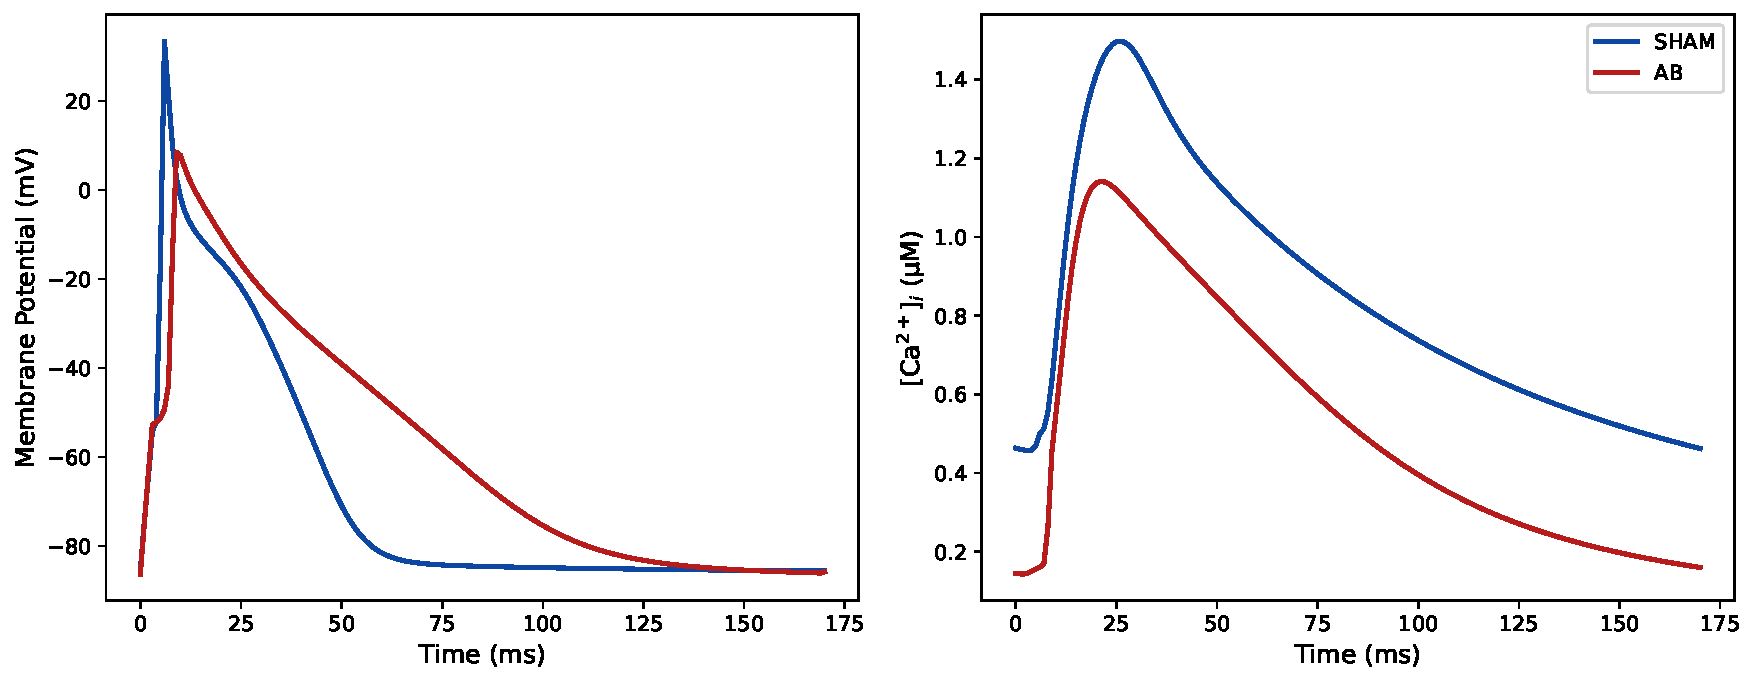
\includegraphics[width=\textwidth]{figures/chapter02/sham_vs_ab_ca_ap.pdf}
    \caption{SHAM (blue) and AB (red) rats characteristic action potentials and calcium transients simulated using the Gattoni et al.~\cite{Gattoni:2017} model of rat left ventricular myocyte electrophysiology at $\SI{6}{\hertz}$ pacing frequency and $\SI{37}{\celsius}$.}
    \label{fig:shamvsabcaap}
\end{figure}


%
%
%
\subsection{Input parameter space}\label{sec:ch4inputparameterspace}
The input parameter space $X\subset\mathbb{R}^{8}$ of the simulator map $f_{simul}$ introduced in equation~\eqref{eq:fsimul} was defined as the Cartesian product of $8$ one-dimensional parameter ranges. These ranges were determined using prior information collected from both experimental and modelling literature studies, summarised in Tables~\ref{tab:shamranges}--\ref{tab:abranges}. The finally adopted parameter ranges are reported in Table~\ref{tab:finalshamabranges}. To avoid bias, we used the same input parameter space $X$ for both the SHAM and AB rat models from where to sample points to be simulated, which are then used to build the emulators' training datasets.

\newpage
\begin{landscape}
\begin{table}
    \vspace{-\marginparsep}
    \vspace{-\marginparwidth}
    \begin{tabularx}{2\textwidth}{llllll}
    \toprule
    \tableheadline{Parameter} & \tableheadline{Units} & \multicolumn{2}{l}{\spacedlowsmallcaps{Value from experimental studies}} & \multicolumn{2}{l}{\spacedlowsmallcaps{Value from modelling studies}} \\ \midrule
     & & \tableheadline{Range} & \tableheadline{Reference} & \tableheadline{Range} & \tableheadline{Reference} \\ \midrule
    $\Caif$ & $\SI{}{\micro\Molar}$                 & $-$ & $-$ & $[0.8,\,1.56]$ & \cite{Land:2012*a, Lewalle:2018, Niederer:2006, Wei-Dong-Gao:1994, Gao:1995, Backx:1995} \\
    $\koff$                                & $\SI{}{\per\milli\second}$            & $[0.0013,\,1.2]$ & \cite{Rosenfeld:1985, Tikunova:2004, Davis:2007} & $[0.05,\,0.2]$ & \cite{Land:2012*a, Lewalle:2018, Niederer:2006} \\
    $\kxb$                                  & $\SI{}{\per\milli\second}$            & $0.1$ & \cite{Blanchard:1999, Stull:2002} & $[0.008,\,0.2]$ & \cite{Land:2012*a, Lewalle:2018} \\
    $\tref$                                 & $\SI{}{\kilo\pascal}$                 & $-$ & $-$ & $[20,\, 160]$ & \cite{Land:2012*a, Lewalle:2018, Niederer:2006, Niederer:2009, Blanchard:1999, Stuyvers:2002, Palmer:2004, Kreutziger:2011, Rice:2008, Bovendeerd:2009} \\
    $\p$                                                & $\SI{}{\kilo\pascal}$                 & $[0.2,\,1.4]$ & \cite{Nemeth:2016, Sato:1990, Schunkert:1995, Loot:2005, Liu:2014, Ku:2014, Ruppert:2018, Schunkert:1990, Ruppert:2016} & $1.0$ & \cite{Land:2012*a, Lewalle:2018} \\
    $\pao$                                              & $\SI{}{\kilo\pascal}$                 & $[12,\,21]$ & \cite{Nemeth:2016, Ku:2014, Ruppert:2018, Kovacs:2015, Lee:2017, Olah:2015, Ruppert:2016, Toledo:2017} & $[8,\,9]$ & \cite{Land:2012*a, Lewalle:2018} \\
    $\Z$                                                & $\SI{}{\mmHg\second\per\milli\litre}$ & $[1.5,\,16]$ & \cite{Kobayashi:1996, Levy:1988, Zuckerman:1989, Lin:2004, Yin:1980, Ioannou:2009, Chang:2015} & $[6,\,20]$ & \cite{Land:2012*a, Lewalle:2018, Westerhof:1991} \\
    $\Cone$                                              & $\SI{}{\kilo\pascal}$                 & $[0.1,\,3.0]$ & \cite{Nordbo:2014} (review paper) & $[0.4,\,1.1]$ & \cite{Land:2012*a, Lewalle:2018, Niederer:2009, Omens:1993} \\
    \bottomrule
    \end{tabularx}
    \caption{SHAM rat model input parameters' values from experimental and modelling studies.}
    \label{tab:shamranges}
\end{table}
\end{landscape}

\newpage
\begin{landscape}
\begin{table}
    \vspace{-\marginparsep}
    \vspace{-\marginparwidth}
    \begin{tabularx}{2\textwidth}{llllll}
    \toprule
    \tableheadline{Parameter} & \tableheadline{Units} & \multicolumn{2}{l}{\spacedlowsmallcaps{Value from experimental studies}} & \multicolumn{2}{l}{\spacedlowsmallcaps{Value from modelling studies}} \\ \midrule
     & & \tableheadline{Range} & \tableheadline{Reference} & \tableheadline{Range} & \tableheadline{Reference} \\ \midrule
    $\Caif$ & $\SI{}{\micro\Molar}$                 & $-$ & $-$ & $[0.8,\,1.0]$ & \cite{Lewalle:2018} \\
    $\koff$                                & $\SI{}{\per\milli\second}$            & $-$ & $-$ & $0.1$ & \cite{Lewalle:2018} \\
    $\kxb$                                  & $\SI{}{\per\milli\second}$            & $-$ & $-$ & $0.02$ & \cite{Lewalle:2018} \\
    $\tref$                                 & $\SI{}{\kilo\pascal}$                 & $-$ & $-$ & $120$ & \cite{Lewalle:2018} \\
    $\p$                                                & $\SI{}{\kilo\pascal}$                 & $[0.3,\,1.6]$ & \cite{Nemeth:2016, Sato:1990, Schunkert:1995, Loot:2005, Liu:2014, Ku:2014, Ruppert:2018, Schunkert:1990, Ruppert:2016} & $1.0$ & \cite{Lewalle:2018} \\
    $\pao$                                              & $\SI{}{\kilo\pascal}$                 & $[21,\,26]$ & \cite{Nemeth:2016, Ku:2014, Ruppert:2018, Ruppert:2016} & $[7,\,20]$ & \cite{Lewalle:2018} \\
    $\Z$                                                & $\SI{}{\mmHg\second\per\milli\litre}$ & $[5.5,\,23]$ & \cite{Kobayashi:1996, Yin:1980, Ioannou:2009} & $9.5$ & \cite{Lewalle:2018} \\
    $\Cone$                                              & $\SI{}{\kilo\pascal}$                 & $-$ & $-$ & $[0.2,\,1.6]$ & \cite{Lewalle:2018} \\
    \bottomrule
    \end{tabularx}
    \caption{AB rat model input parameters' values from experimental and modelling studies.}
    \label{tab:abranges}
\end{table}
\end{landscape}

\newpage
\begin{table}[!ht]
    \myfloatalign
    \begin{tabularx}{\textwidth}{XXX}
        \toprule
        \tableheadline{Parameter} & \tableheadline{Units} & \tableheadline{Range} \\
        \midrule
        $\Caif$ & $\SI{}{\micro\Molar\tothe{1/2}}$      & $[0.25,\,3.25]$ \\
        $\koff$ & $\SI{}{\per\milli\second}$            & $[0.05,\,0.2]$ \\
        $\kxb$  & $\SI{}{\per\milli\second}$            & $[0.008,\,0.2]$ \\
        $\tref$ & $\SI{}{\kilo\pascal}$                 & $[80,\,160]$ \\
        $\p$    & $\SI{}{\kilo\pascal}$                 & $[0.3,\,1.4]$ \\
        $\pao$  & $\SI{}{\kilo\pascal}$                 & $[6,\,21]$ \\
        $\Z$    & $\SI{}{\mmHg\second\per\milli\litre}$ & $[5.5,\,20]$ \\
        $\Cone$ & $\SI{}{\kilo\pascal}$                 & $[0.1,\,3]$ \\
        \bottomrule
    \end{tabularx}
    \caption{Input parameter ranges used for both the SHAM and AB rat models.}
    \label{tab:finalshamabranges}
\end{table}


%
%
%
\subsection{Training dataset and emulators}\label{sec:ch4trainingdatasetandemulators}
We trained GPEs on model simulations to replace the simulator multi-scale map (Section~\ref{sec:ch3multiscalemap}) with a fast-evaluating map. GPEs were defined as the sum of a linear regression model and a zero-mean GP, as described in Section~\ref{sec:ch3gaussianprocessemulation}, although for this study the learning sample was modelled not to be noisy. The GPE training was performed in two steps as described previously~\cite{Vernon:2010,Vernon:2018}. Firstly, the linear regression model's coefficients were fitted to the data by minimising the residual sum of squares; secondly, the GP's hyperparameters were fitted to the residuals (data minus predicted mean) by maximisation of the log-marginal likelihood function (equation~\eqref{eq:logmarginallikelihood} with $H_{X}\beta=0$ and $\sigma_n^2=0$). GPEs' were implemented and the training was performed using \texttt{scikit-learn} Python library~\cite{Pedregosa:2011}.

\vspace{0.2cm}
The emulation framework is outlined in Figure~\ref{fig:emulatorframework}. Briefly, $8$ LHDs of $1,024$ input parameter points each were simulated and the successfully completed simulations were collected to form the training dataset, with final size of $825$ and $850$ points for the SHAM and AB models, respectively. The low number of successful runs relates to a combination of failure of the mechanics simulations converging or completing a full cardiac cycle, which may happen if the contraction is insufficient to reach the aortic pressure. One GPE was then trained for each LV output feature (Table~\ref{tab:lvfeatures}), for a total of $12$ GPEs. 

\begin{figure}[!ht]
    \myfloatalign
    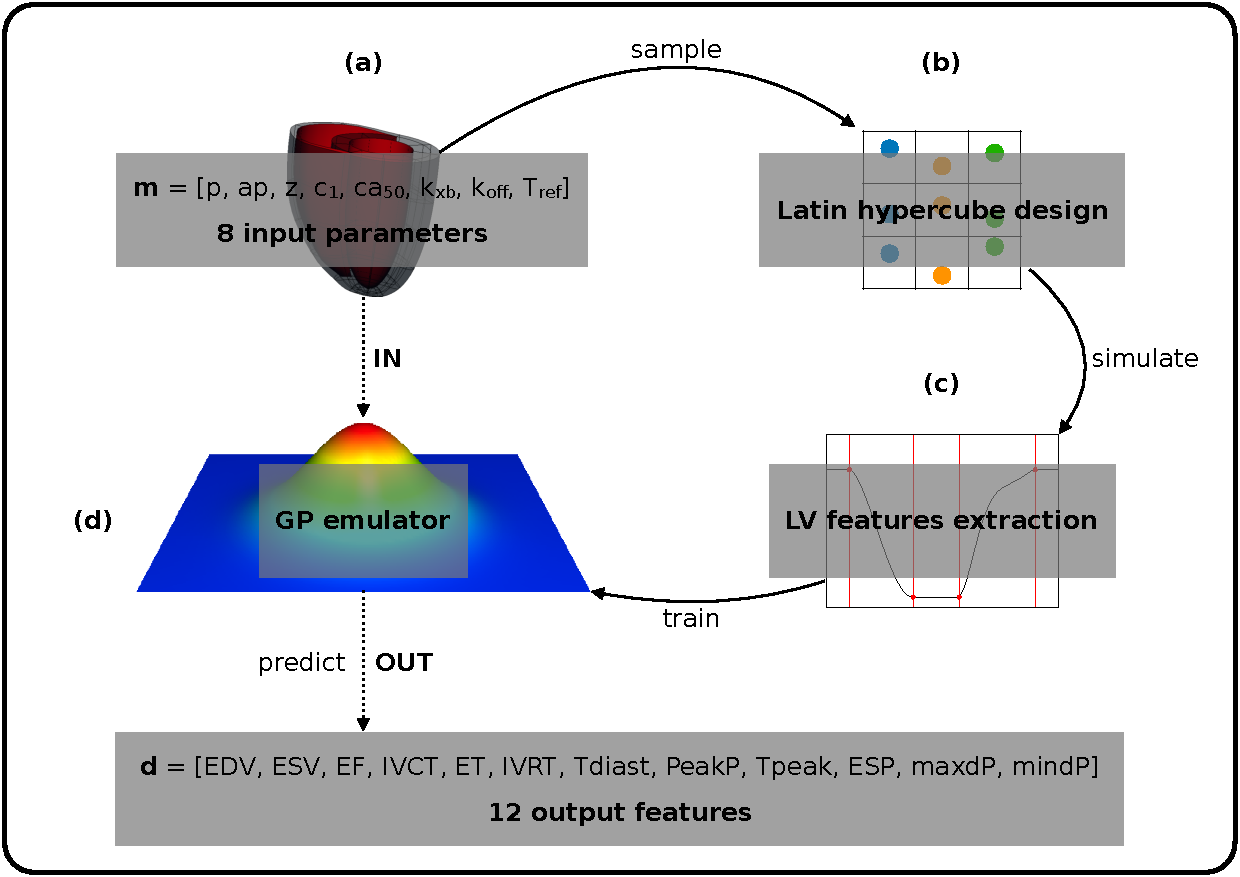
\includegraphics[width=\textwidth]{figures/chapter04/emulator_framework.pdf}
    \caption{Building the surrogate model. Input points (a) are sampled in the parameter space using a Latin hypercube design (b). The model (simulator) is run using these points. The simulator output is composed of features extracted from the LV volume and pressure transients and PV loop (c). The initial input matrix and the corresponding output matrix represent the training dataset for the surrogate model (emulator) based on Gaussian processes. The trained emulator (d) is used to predict the simulator output at a new point in the input parameter space. \todo{renew figure}}
    \label{fig:emulatorframework}
\end{figure}

\vspace{0.2cm}
The trained GPEs were firstly employed to perform a global sensitivity analysis. A subset of them was then used in combination with the experimental target values to fit the rat models.


%
%
%
\subsection{Global sensitivity analysis}
To assess how uncertainty in the model's output can be attributed to different sources of uncertainty in the model input factors, we performed a variance-based sensitivity analysis. Variance-based methods of probabilistic sensitivity analysis quantify the sensitivity of the output to the model inputs in terms of a reduction in the variance of the output. We measured this reduction by estimating the Sobol' sensitivity indices~\cite{Sobol:2001} as described in Section~\ref{sec:ch3estimatingsobolsensitivityindices}.

\vspace{0.2cm}
Sobol' sensitivity indices were estimated using the \texttt{SALib} Python library~\cite{Herman:2017}, integrated with GPEs' posterior mean point-wise predictions, according to the first emulation-based approach of equation~\eqref{eq:emulmeangsa}, presented in Section~\ref{sec:ch3emulatorbasedestimates}. Parameters whose Sobol' indices' distributions' expectation was below the threshold $0.01$ were determined to have negligible effects.


%
%
%
\subsection{History matching}\label{sec:ch4historymatching}
The \textit{in silico} rat heart biophysical model should aim to achieve the best representation of the real system. This requires tuning the model input parameters such that the model output features reflect the available experimental data.

\vspace{0.2cm}
We constrained the model parameters based on model read-outs that describe key features in the LV volume and pressure transients, and PV loop (Table~\ref{tab:lvfeatures}). For this purpose, we adopted the HM approach described in Section~\ref{sec:ch3historymatching}. The maximum implausibility measure (equation~\eqref{eq:maximplmeasure}) across multiple target features was used, with the model discrepancy term (and its corresponding variance) set to zero in equation~\eqref{eq:implmeasure}. The real system observation $z$ and the related observation error $\mathbb{V}[e]$ were taken to be equal to the mean $\mu_j$ and the square of the standard deviation $\sigma_j$ characterising the experimental variability $\mu_j\pm\sigma_j\in\mathbb{R}$ of each given $j$-th feature.

\vspace{0.2cm}
Target features' mean and standard deviation experimental values to match came from two different sources. Specific organ-scale feature unavailable in the MRI data \cite{Roe:2017} were deduced from literature experimental studies all performed on male rats at body temperature with abdominal/ascending aortic banding~\cite{Nemeth:2016, Sato:1990, Schunkert:1995, Loot:2005, Liu:2014, Ku:2014, Ruppert:2018, Schunkert:1990, Ruppert:2016}. In particular, EDV, ESV, ET and IVRT features were immediately available from the MRI data, while information about PeakP, maxdP and mindP features was collected from literature. We did not have specific values for IVCT, Tdiast, Tpeak and ESP, and we chose not to match EF explicitly as this is derived from EDV and ESV. This gave us $7$ organ-scale features to constrain our model parameters. Their experimental variability is reported in Table~\ref{tab:values2match}.

\begin{table}[!ht]
    \myfloatalign
    \begin{tabularx}{\textwidth}{lrrl}
    \toprule
    \tableheadline{LV feature} & \multicolumn{2}{c}{\spacedlowsmallcaps{Exp. variability}} & \tableheadline{Reference} \\
    \midrule
    & \tableheadline{SHAM} & \tableheadline{AB} & \\
    \midrule
    $\textrm{EDV}^{*}$                  & $508.80 \pm 39.01$ & $466.50 \pm 37.10$ & \cite{Roe:2017} \\
    $\textrm{ESV}^{*}$                  & $154.60 \pm 16.53$ & $125.60 \pm 23.40$ & \cite{Roe:2017} \\
    $\textrm{ET}^{*}$                 & $51.21  \pm  1.85$ & $54.72  \pm  1.85$ & \cite{Roe:2017} \\
    $\textrm{IVRT}^{*}$                 & $20.55  \pm  1.85$ & $41.11  \pm  1.85$ & \cite{Roe:2017} \\
    $\textrm{PeakP}^{**}$                  & $16.66  \pm  1.02$ & $21.66  \pm  0.69$ & \cite{Sato:1990, Schunkert:1990, Schunkert:1995, Loot:2005, Ku:2014, Liu:2014, Nemeth:2016, Ruppert:2016, Ruppert:2018} \\
    $\textrm{maxdP}^{**}$ & $1.14   \pm  0.25$ & $1.24   \pm  0.24$ & \cite{Sato:1990, Schunkert:1990, Schunkert:1995, Loot:2005, Ku:2014, Liu:2014, Nemeth:2016, Ruppert:2016, Ruppert:2018} \\
    $\textrm{mindP}^{**}$ & $-1.00  \pm  0.23$ & $-1.16  \pm  0.23$ & \cite{Sato:1990, Schunkert:1990, Schunkert:1995, Loot:2005, Ku:2014, Liu:2014, Nemeth:2016, Ruppert:2016, Ruppert:2018} \\
    \bottomrule
    \end{tabularx}
    \caption{Left ventricular features' target mean and standard deviation values. One asterisk $(\,\,)^*$ features values come directly from the available MRI data. Two asterisks $(\,\,)^{**}$ features values come from literature experimental studies.}
    \label{tab:values2match}
\end{table}

\vspace{0.2cm}
The HM was performed as follows. We started with $400,000$ $NROY$ points for wave $1$, sampled using a Latin hypercube design in the input parameter space $X$ (defined in Section~\ref{sec:ch4inputparameterspace}). For the next waves, $50,000$ $NROY$ points were sampled using the cloud technique in the corresponding previous waves' non-implausible space $X_{NIMP}$. At each wave, $256$ points were selected from the current $X_{NIMP}$ space using the part-and-select algorithm and simulated to enrich the training dataset for the next wave's emulators.

\vspace{0.2cm}
The cutoff value $I_{\,\text{cutoff}}$ was initialised to $3.0$, and incremented by $0.5$ units until we achieved a non-empty non-implausible set after applying the implausibility criterion using the first wave's emulators. This gave initial $I_{\,\text{cutoff}}s$ of $5.5$ and $5.0$ for the SHAM and AB rat models’ fitting, respectively. $I_{\,\text{cutoff}}$ was then decremented by $0.5$ units with each HM wave down to the commonly used value of $3.0$ (see Section~\ref{sec:ch3historymatching}). The decrement rate of $0.5$ was selected to ensure that we reached the desired final value of $3.0$ within a reasonable number waves, to maintain computational tractability, while allowing us to initialise the HM over a sufficient large search space. The final waves were run with $I_{\,\text{cutoff}}=3.0$.


%
%
%
\section{Results}\label{sec:ch4results}

%
%
%
\subsection{Model emulation}
The obtained cross-validation GPEs' test scores used as a measure of accuracy as described in Section~\ref{sec:ch3gaussianprocessemulation} are reported in Tables~\ref{tab:gpescores1_sham}--\ref{tab:gpescores1_ab} for the SHAM and AB models' emulators, respectively. Each emulator evaluation at a new imput parameter point took $\sim 1.2$ seconds against a full simulator single-core run of $\sim 4$ hours, for a total gained speedup of $12,000$ fold per evaluation. An example illustration of emulators doing inference on a test set from the cross-validation process is provided in Figures~\ref{fig:gpesexampleinferencesham}--\ref{fig:gpesexampleinferenceab} for the SHAM and AB models' emulators, respectively.

\begin{table}[!ht]
    \myfloatalign
    \begin{tabularx}{\textwidth}{XXX}
    \toprule
    \tableheadline{LV feature} & \tableheadline{$R^2$} & \tableheadline{$ISE_2 (\SI{}{\percent})$} \\
    \midrule
    $\textrm{EDV}$    & $0.9712 \pm 0.0046$ & $87.75 \pm 1.17$ \\
    $\textrm{ESV}$    & $0.9736 \pm 0.0023$ & $86.42 \pm 2.53$ \\
    $\textrm{EF}$     & $0.9342 \pm 0.0155$ & $87.63 \pm 2.44$ \\
    $\textrm{IVCT}$   & $0.9658 \pm 0.0122$ & $88.00 \pm 4.50$ \\
    $\textrm{ET}$     & $0.9408 \pm 0.0054$ & $88.24 \pm 1.65$ \\
    $\textrm{IVRT}$   & $0.9135 \pm 0.0128$ & $87.63 \pm 4.38$ \\
    $\textrm{Tdiast}$ & $0.9412 \pm 0.0056$ & $86.66 \pm 1.99$ \\
    $\textrm{PeakP}$  & $0.9867 \pm 0.0027$ & $86.78 \pm 1.04$ \\
    $\textrm{Tpeak}$  & $0.9659 \pm 0.0117$ & $85.69 \pm 5.82$ \\
    $\textrm{ESP}$    & $0.9973 \pm 0.0004$ & $86.66 \pm 2.23$ \\
    $\textrm{maxdP}$  & $0.9792 \pm 0.0064$ & $86.66 \pm 4.89$ \\
    $\textrm{mindP}$  & $0.7437 \pm 0.0283$ & $93.45 \pm 1.64$ \\
    \bottomrule
    \end{tabularx}
    \caption{The SHAM rat GPEs' accuracy. The GPEs' accuracy was evaluated using the average $R^{2}$ score and $ISE_2$ obtained with a $5$-fold cross-validation. Values are reported as mean$\pm$std.}
    \label{tab:gpescores1_sham}
\end{table}

\begin{table}[!ht]
    \myfloatalign
    \begin{tabularx}{\textwidth}{XXX}
    \toprule
    \tableheadline{LV feature} & \tableheadline{$R^2$} & \tableheadline{$ISE_2 (\SI{}{\percent})$} \\
    \midrule
    $\textrm{EDV}$    & $0.9461 \pm 0.0273$ & $87.88 \pm 4.05$ \\
    $\textrm{ESV}$    & $0.9714 \pm 0.0050$ & $87.29 \pm 2.37$ \\
    $\textrm{EF}$     & $0.9661 \pm 0.0101$ & $86.23 \pm 3.63$ \\
    $\textrm{IVCT}$   & $0.9906 \pm 0.0021$ & $84.47 \pm 2.51$ \\     
    $\textrm{ET}$     & $0.9593 \pm 0.0159$ & $89.29 \pm 3.49$ \\
    $\textrm{IVRT}$   & $0.8559 \pm 0.0165$ & $85.88 \pm 1.78$ \\
    $\textrm{Tdiast}$ & $0.9473 \pm 0.0197$ & $88.11 \pm 4.06$ \\
    $\textrm{PeakP}$  & $0.9871 \pm 0.0077$ & $85.29 \pm 2.13$ \\
    $\textrm{Tpeak}$  & $0.9542 \pm 0.0150$ & $86.00 \pm 7.70$ \\
    $\textrm{ESP}$    & $0.9959 \pm 0.0024$ & $86.23 \pm 2.59$ \\
    $\textrm{maxdP}$  & $0.9860 \pm 0.0039$ & $87.41 \pm 3.08$ \\
    $\textrm{mindP}$  & $0.7474 \pm 0.0687$ & $89.76 \pm 2.37$ \\
    \bottomrule
    \end{tabularx}
    \caption{The AB rat GPEs' accuracy. The GPEs' accuracy was evaluated using the average $R^{2}$ score and $ISE_2$ obtained with a $5$-fold cross-validation. Values are reported as mean$\pm$std.}
    \label{tab:gpescores1_ab}
\end{table}

\begin{figure}[!ht]
    \myfloatalign
    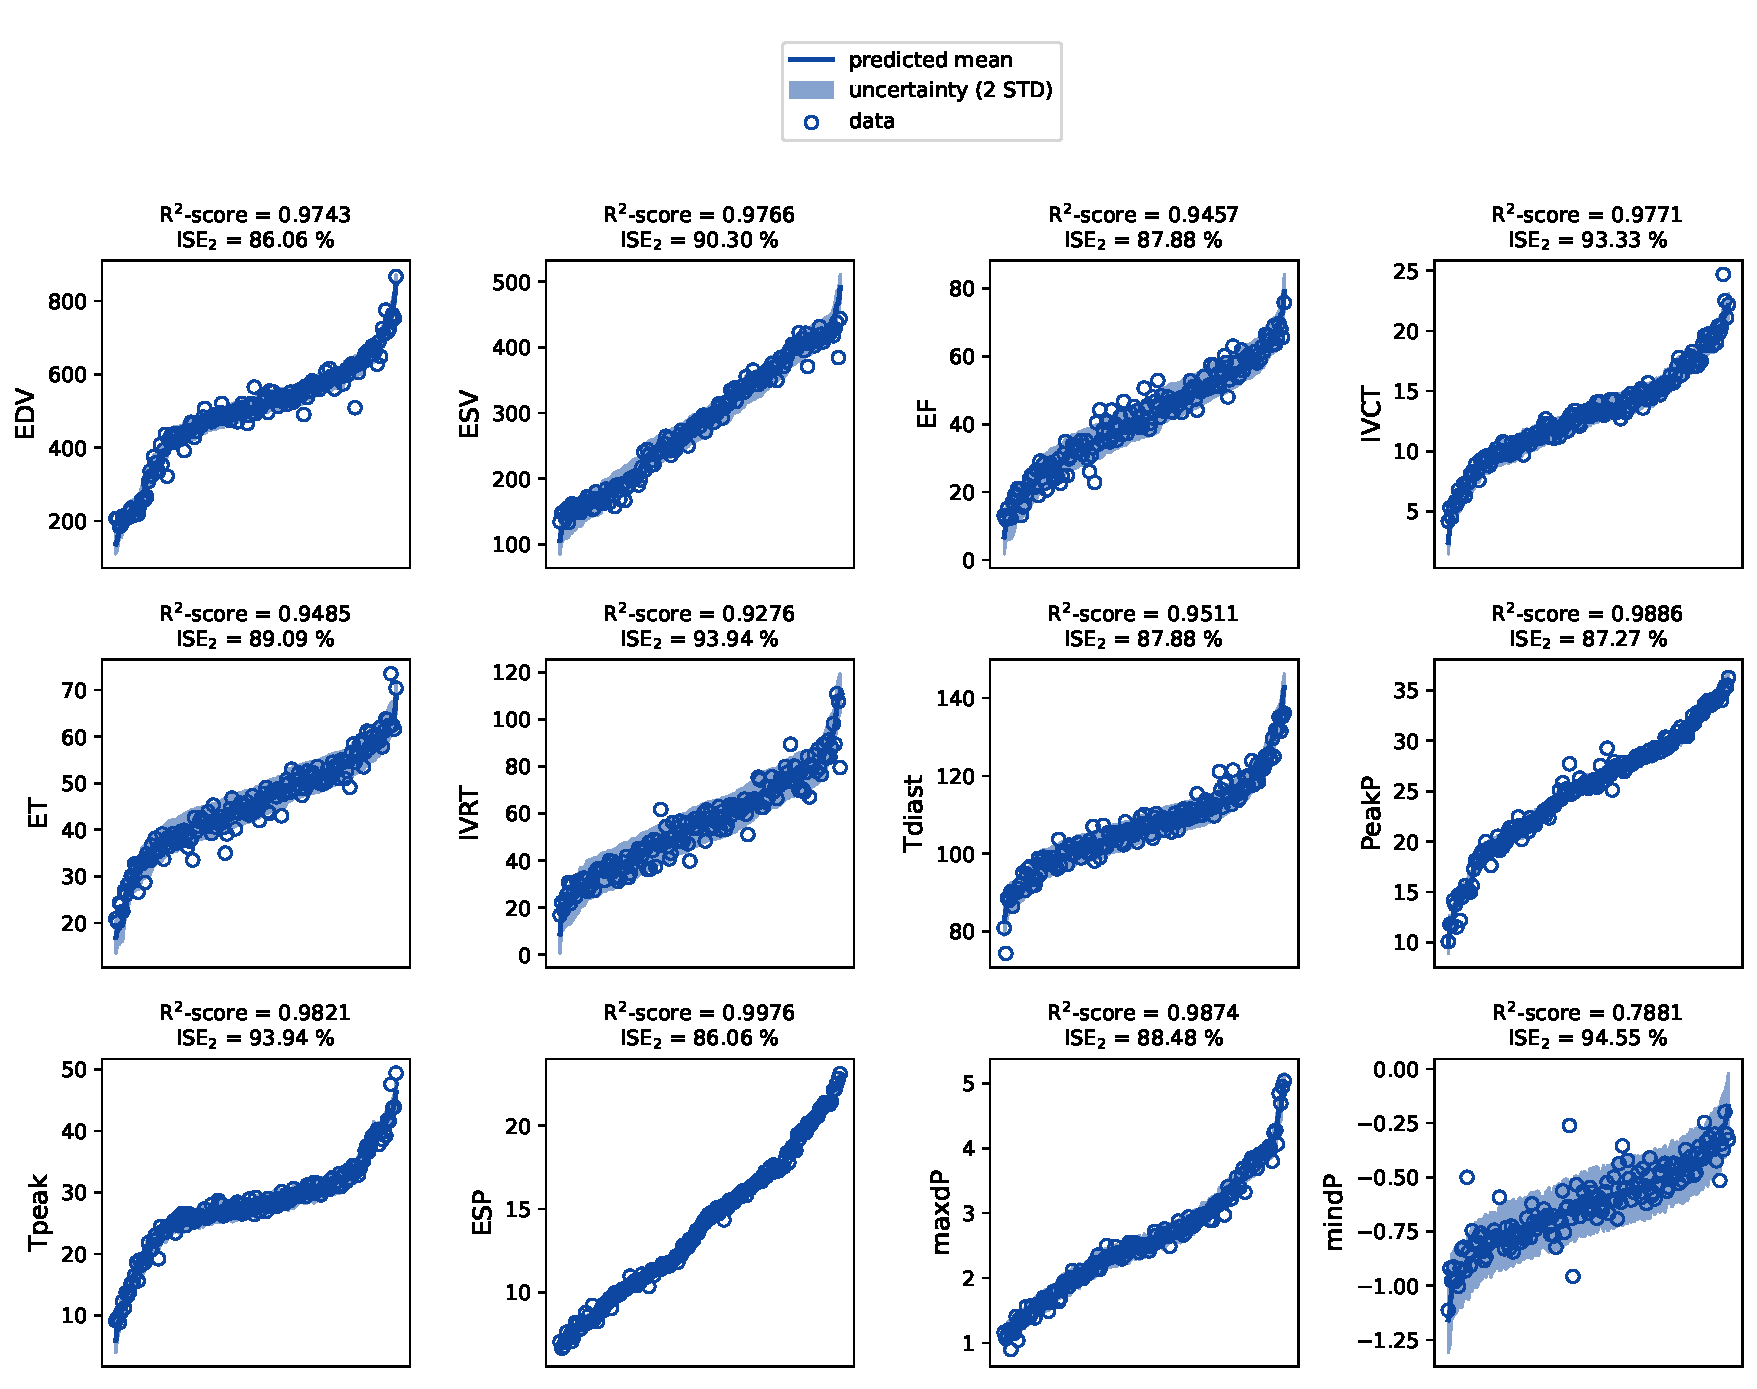
\includegraphics[width=\textwidth]{figures/chapter04/bgpes_vs_bsplit_sham.pdf}
    \caption{For each LV feature, the GPE with the highest $R^2$ split test score is used to make predictions at the respective left-out subset of test points. Predictions are sorted in ascending order for the sake of a better visualisation and joined with a thick blue line, and the respective observations (empty dots) are sorted accordingly. $2$ STD confidence intervals (shaded regions) are also plotted around predicted mean lines.}
    \label{fig:gpesexampleinferencesham}
\end{figure}

\begin{figure}[!ht]
    \myfloatalign
    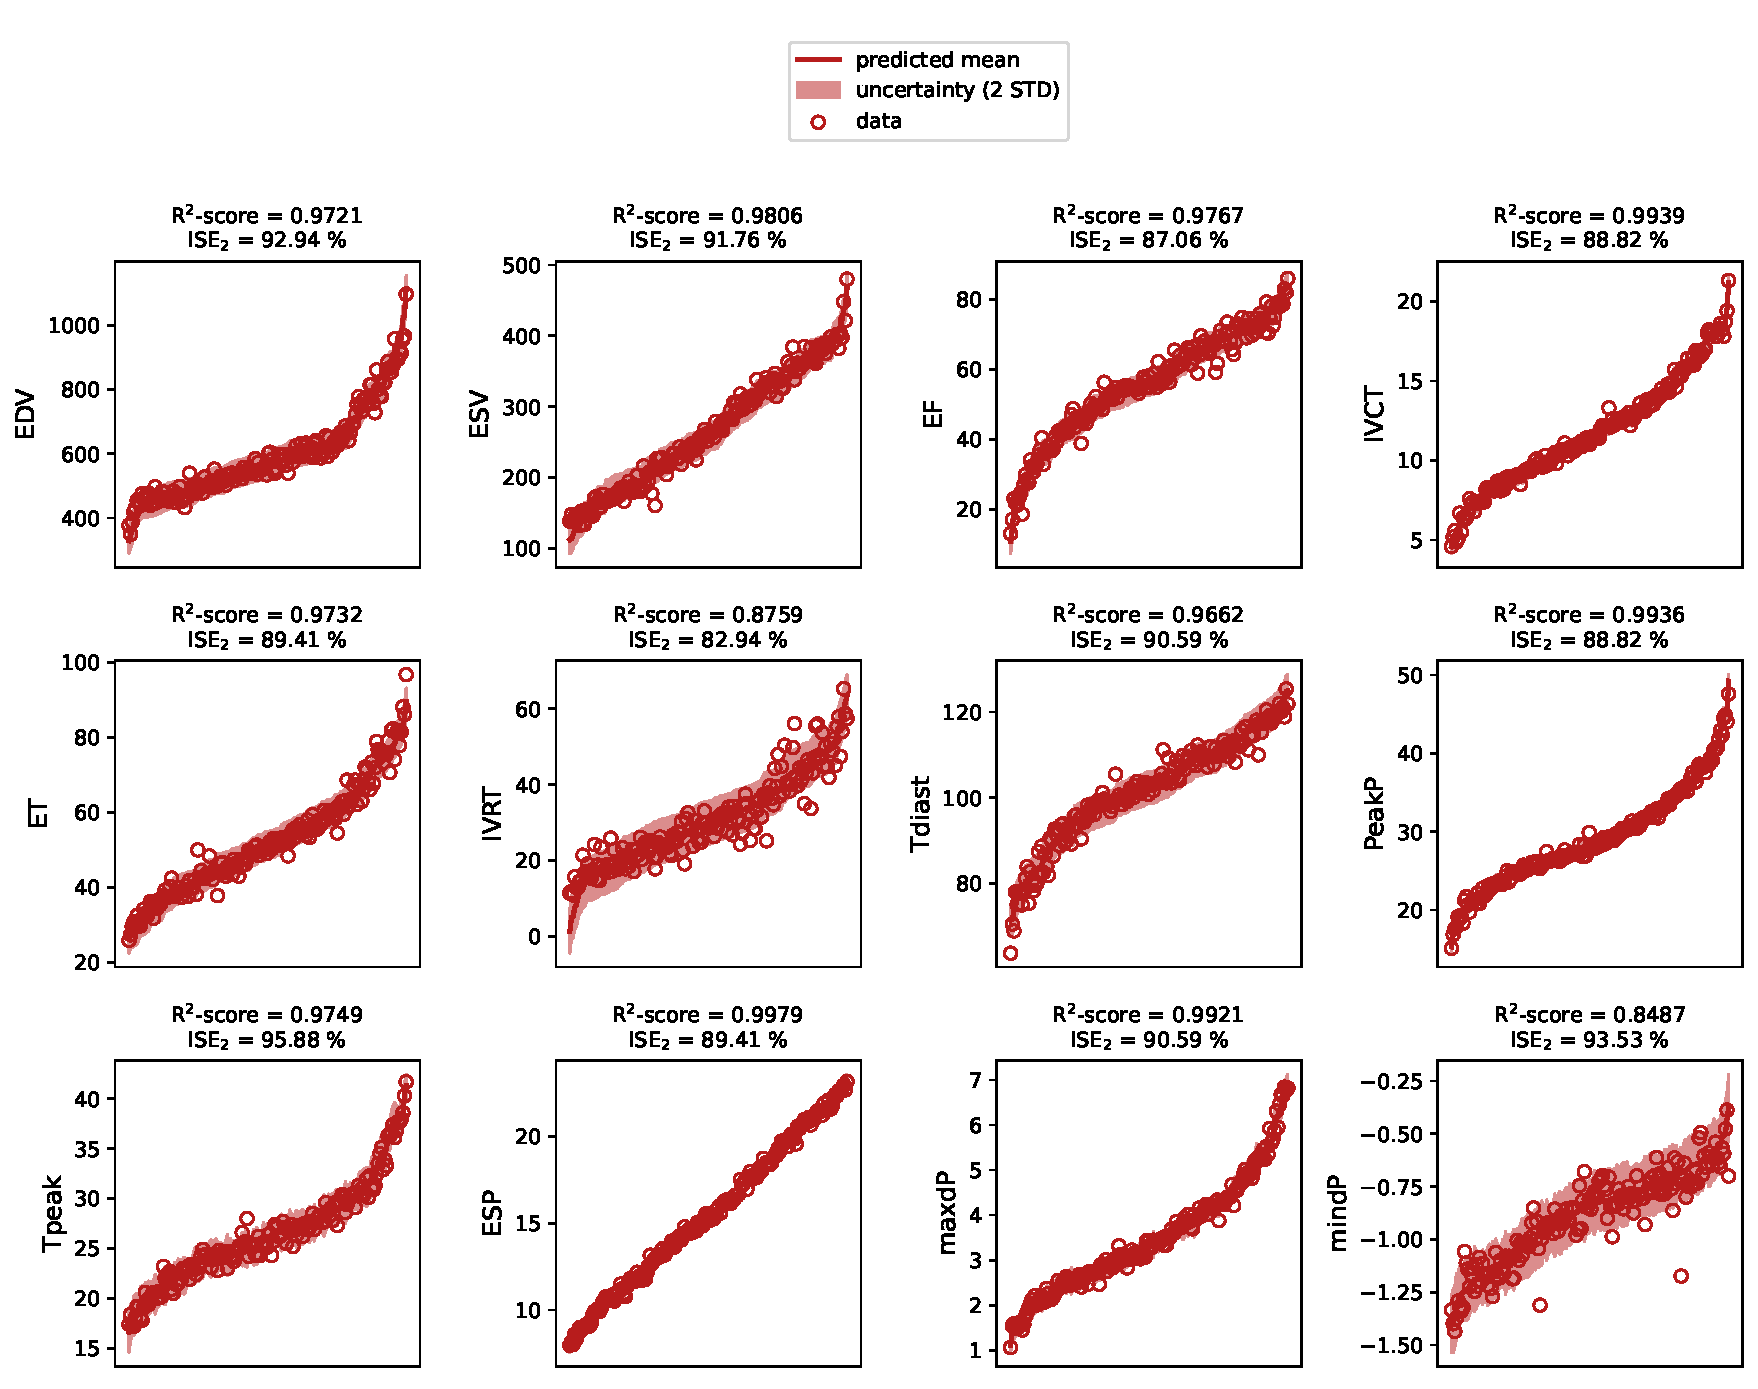
\includegraphics[width=\textwidth]{figures/chapter04/bgpes_vs_bsplit_ab.pdf}
    \caption{For each LV feature, the GPE with the highest $R^2$ split test score is used to make predictions at the respective left-out subset of test points. Predictions are sorted in ascending order for the sake of a better visualisation and joined with a thick blue line, and the respective observations (empty dots) are sorted accordingly. $2$ STD confidence intervals (shaded regions) are also plotted around predicted mean lines.}
    \label{fig:gpesexampleinferenceab}
\end{figure}


%
%
%
\subsection{Model output sensitivity to model input}
Figures~\ref{fig:shamgsa}--\ref{fig:abgsa} show how input parameters contribute to explaining each LV feature's total variance in the SHAM and AB models.

\begin{figure}[!ht]
    \myfloatalign
    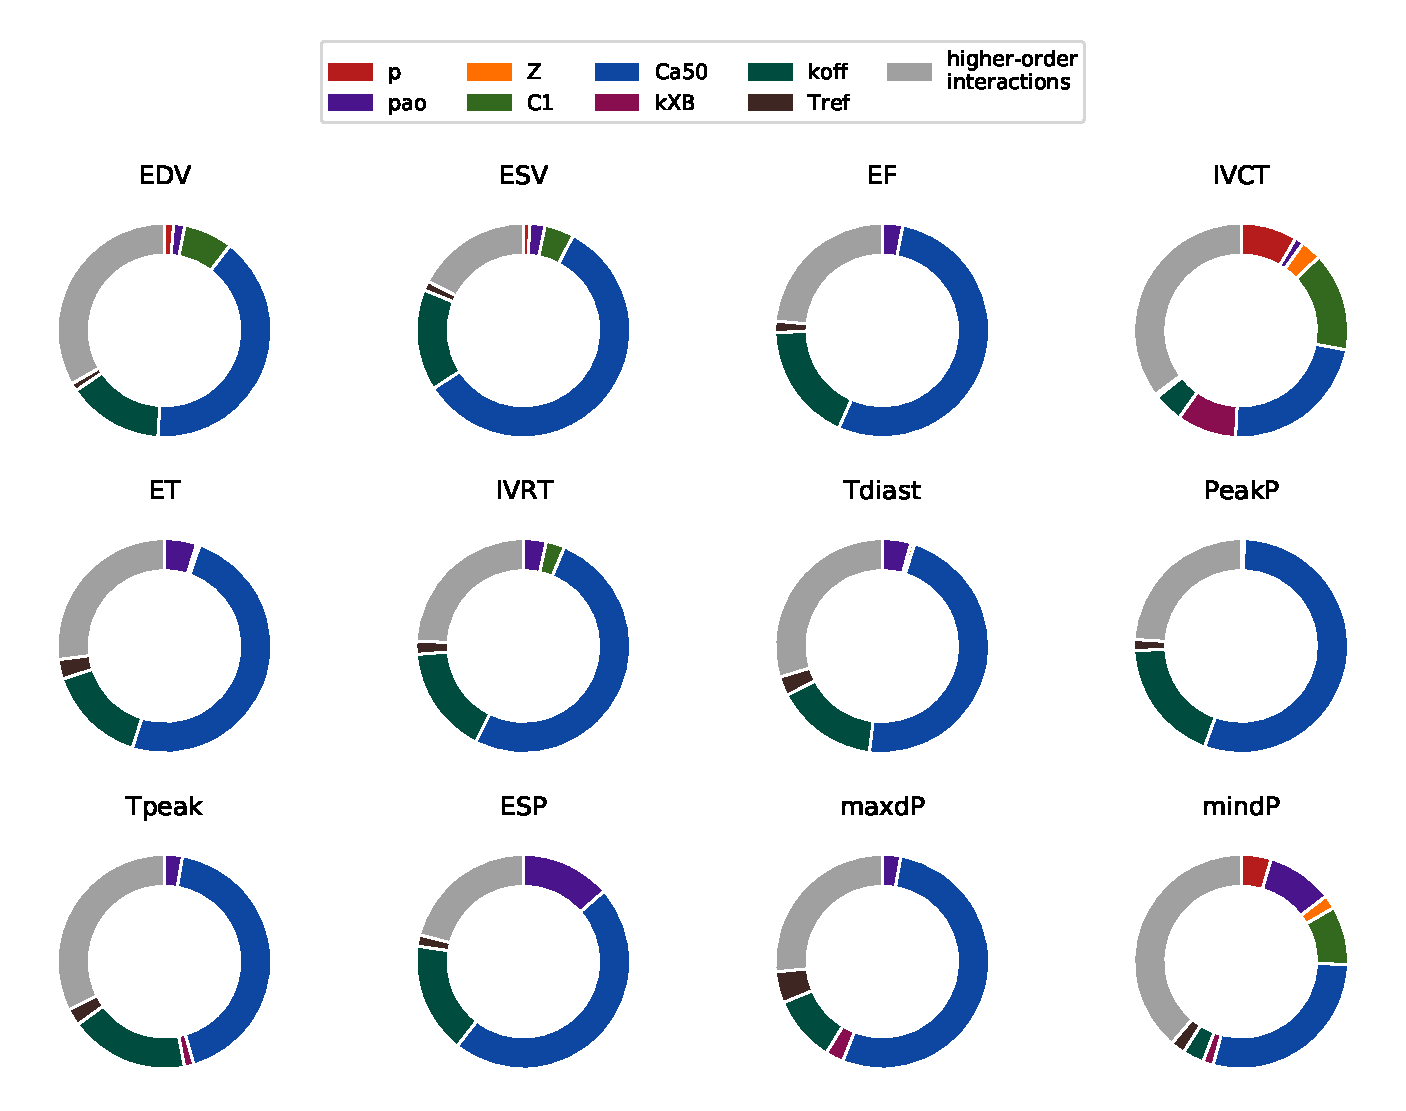
\includegraphics[width=\textwidth]{figures/chapter04/gsa_sham.pdf}
    \caption{The impact of cell, tissue and boundary conditions properties on organ-scale LV features in the SHAM rat model. The contribution of each parameter is represented by the sum of its first- and (when present) second-order effects. For each LV feature, higher-order interactions (coloured in grey) are represented by the sum of total effects minus the sum of all first- and second-order effects.}
    \label{fig:shamgsa}
\end{figure}

\begin{figure}[!ht]
    \myfloatalign
    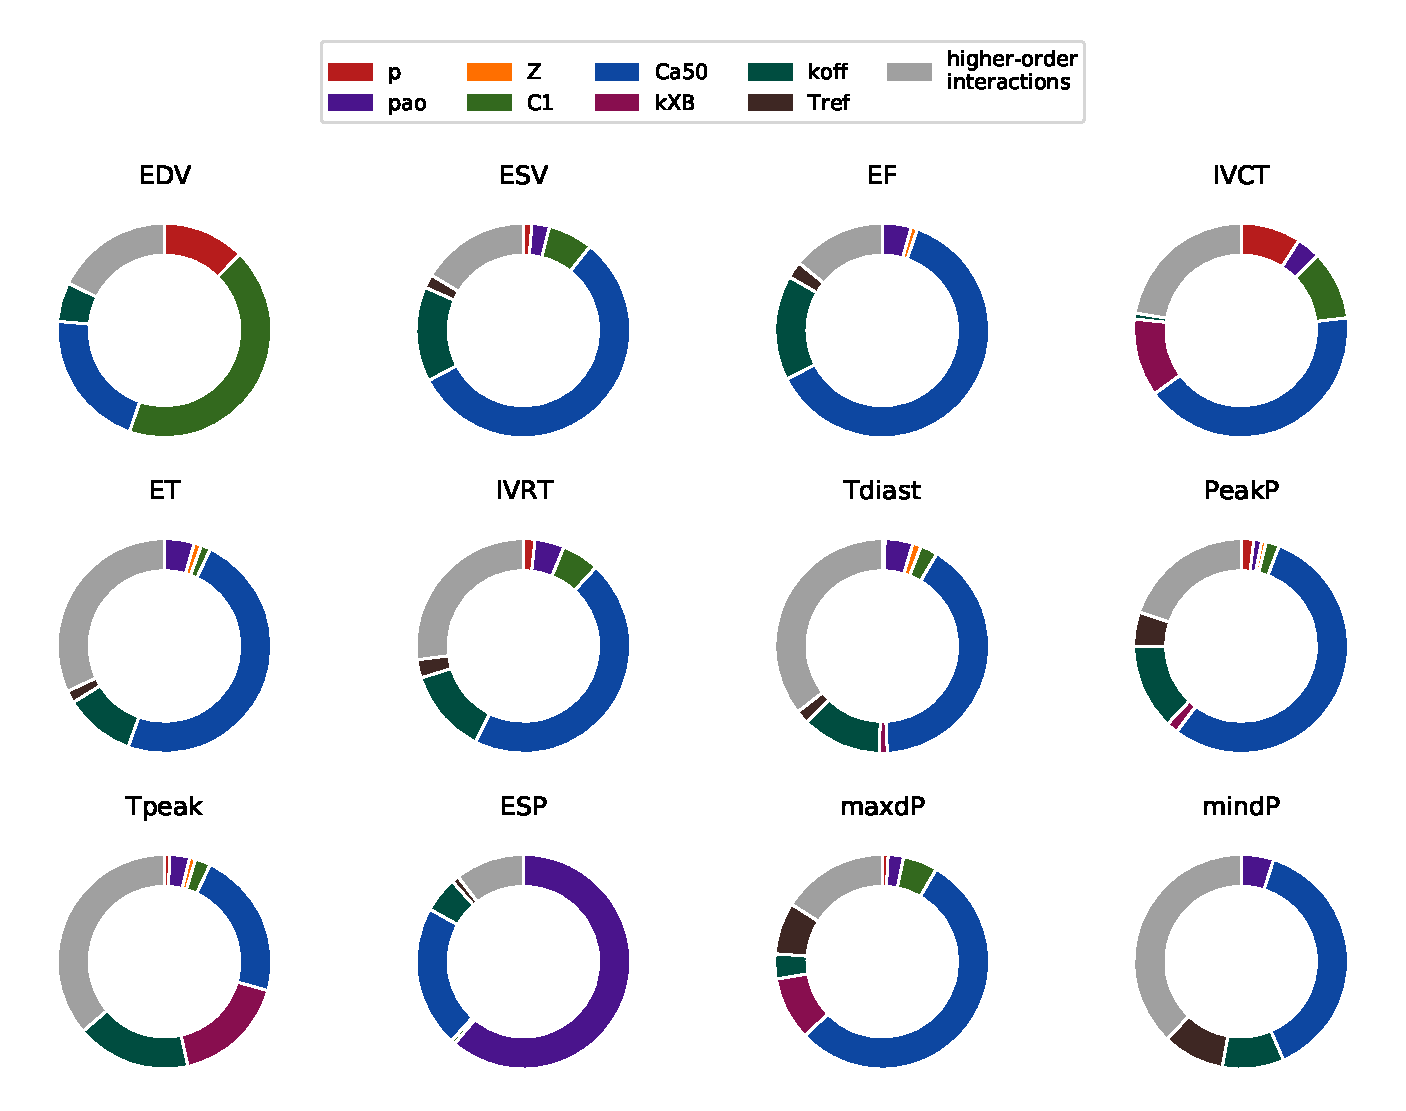
\includegraphics[width=\textwidth]{figures/chapter04/gsa_ab.pdf}
    \caption{The impact of cell, tissue and boundary conditions properties on organ-scale LV features in the AB rat model. The contribution of each parameter is represented by the sum of its first- and (when present) second-order effects. For each LV feature, higher-order interactions (coloured in grey) are represented by the sum of total effects minus the sum of all first- and second-order effects.}
    \label{fig:abgsa}
\end{figure}

\noindent
The $\Caif$ parameter is the most influential across all the LV features. The $\koff$, $\tref$ and $\pao$ parameters also play a key role. All these statements are true for both rat phenotypes. In contrast, $\Cone$ is more important for AB than for SHAM, explaining a fraction of the total variance of $9$ out of $12$ LV features (in SHAM, $\Cone$ is important for only $5$ features). In particular, this parameter has an important contribution in explaining end-diastolic volume in AB (and not in SHAM). The $\kxb$ parameter affects the AB more than the SHAM features, albeit only moderately ($5$ out of $12$ against $4$ out of $12$, respectively). Finally, we observe an increased contribution of $\pao$ in explaining end-systolic pressure when going from SHAM to AB.


%
%
%
\subsection{Model fitting}\label{sec:ch4modelfitting}
The HM process is illustrated in Figures~\ref{fig:shamhm}--\ref{fig:abhm} for the SHAM and AB rat models. The input parameter points in $8$D are plotted as a $2$D projection for each pair of parameters. The initial $X$ space (lightest colour variants) became progressively constrained to smaller $X_{NIMP}$ regions (darker colour variants) as the HM process went forward. During the last waves, as we continued to observe a decrease in the $X_{NIMP}$ space volume, we stopped the process when the percentage of $X_{NIMP}$ points out of the total testing $NROY$ points fell below $\SI{5}{\percent}$. This prevented exhaustion of computational resources, although convergence of the $X_{NIMP}$ space had not yet been reached, completing SHAM and AB models' fitting in $8$ and $9$ waves, respectively. Details of HM progression including cutoff values and percentages of space reduction are given in Table~\ref{tab:hmdetails}.

\begin{figure}[!ht]
    \myfloatalign
    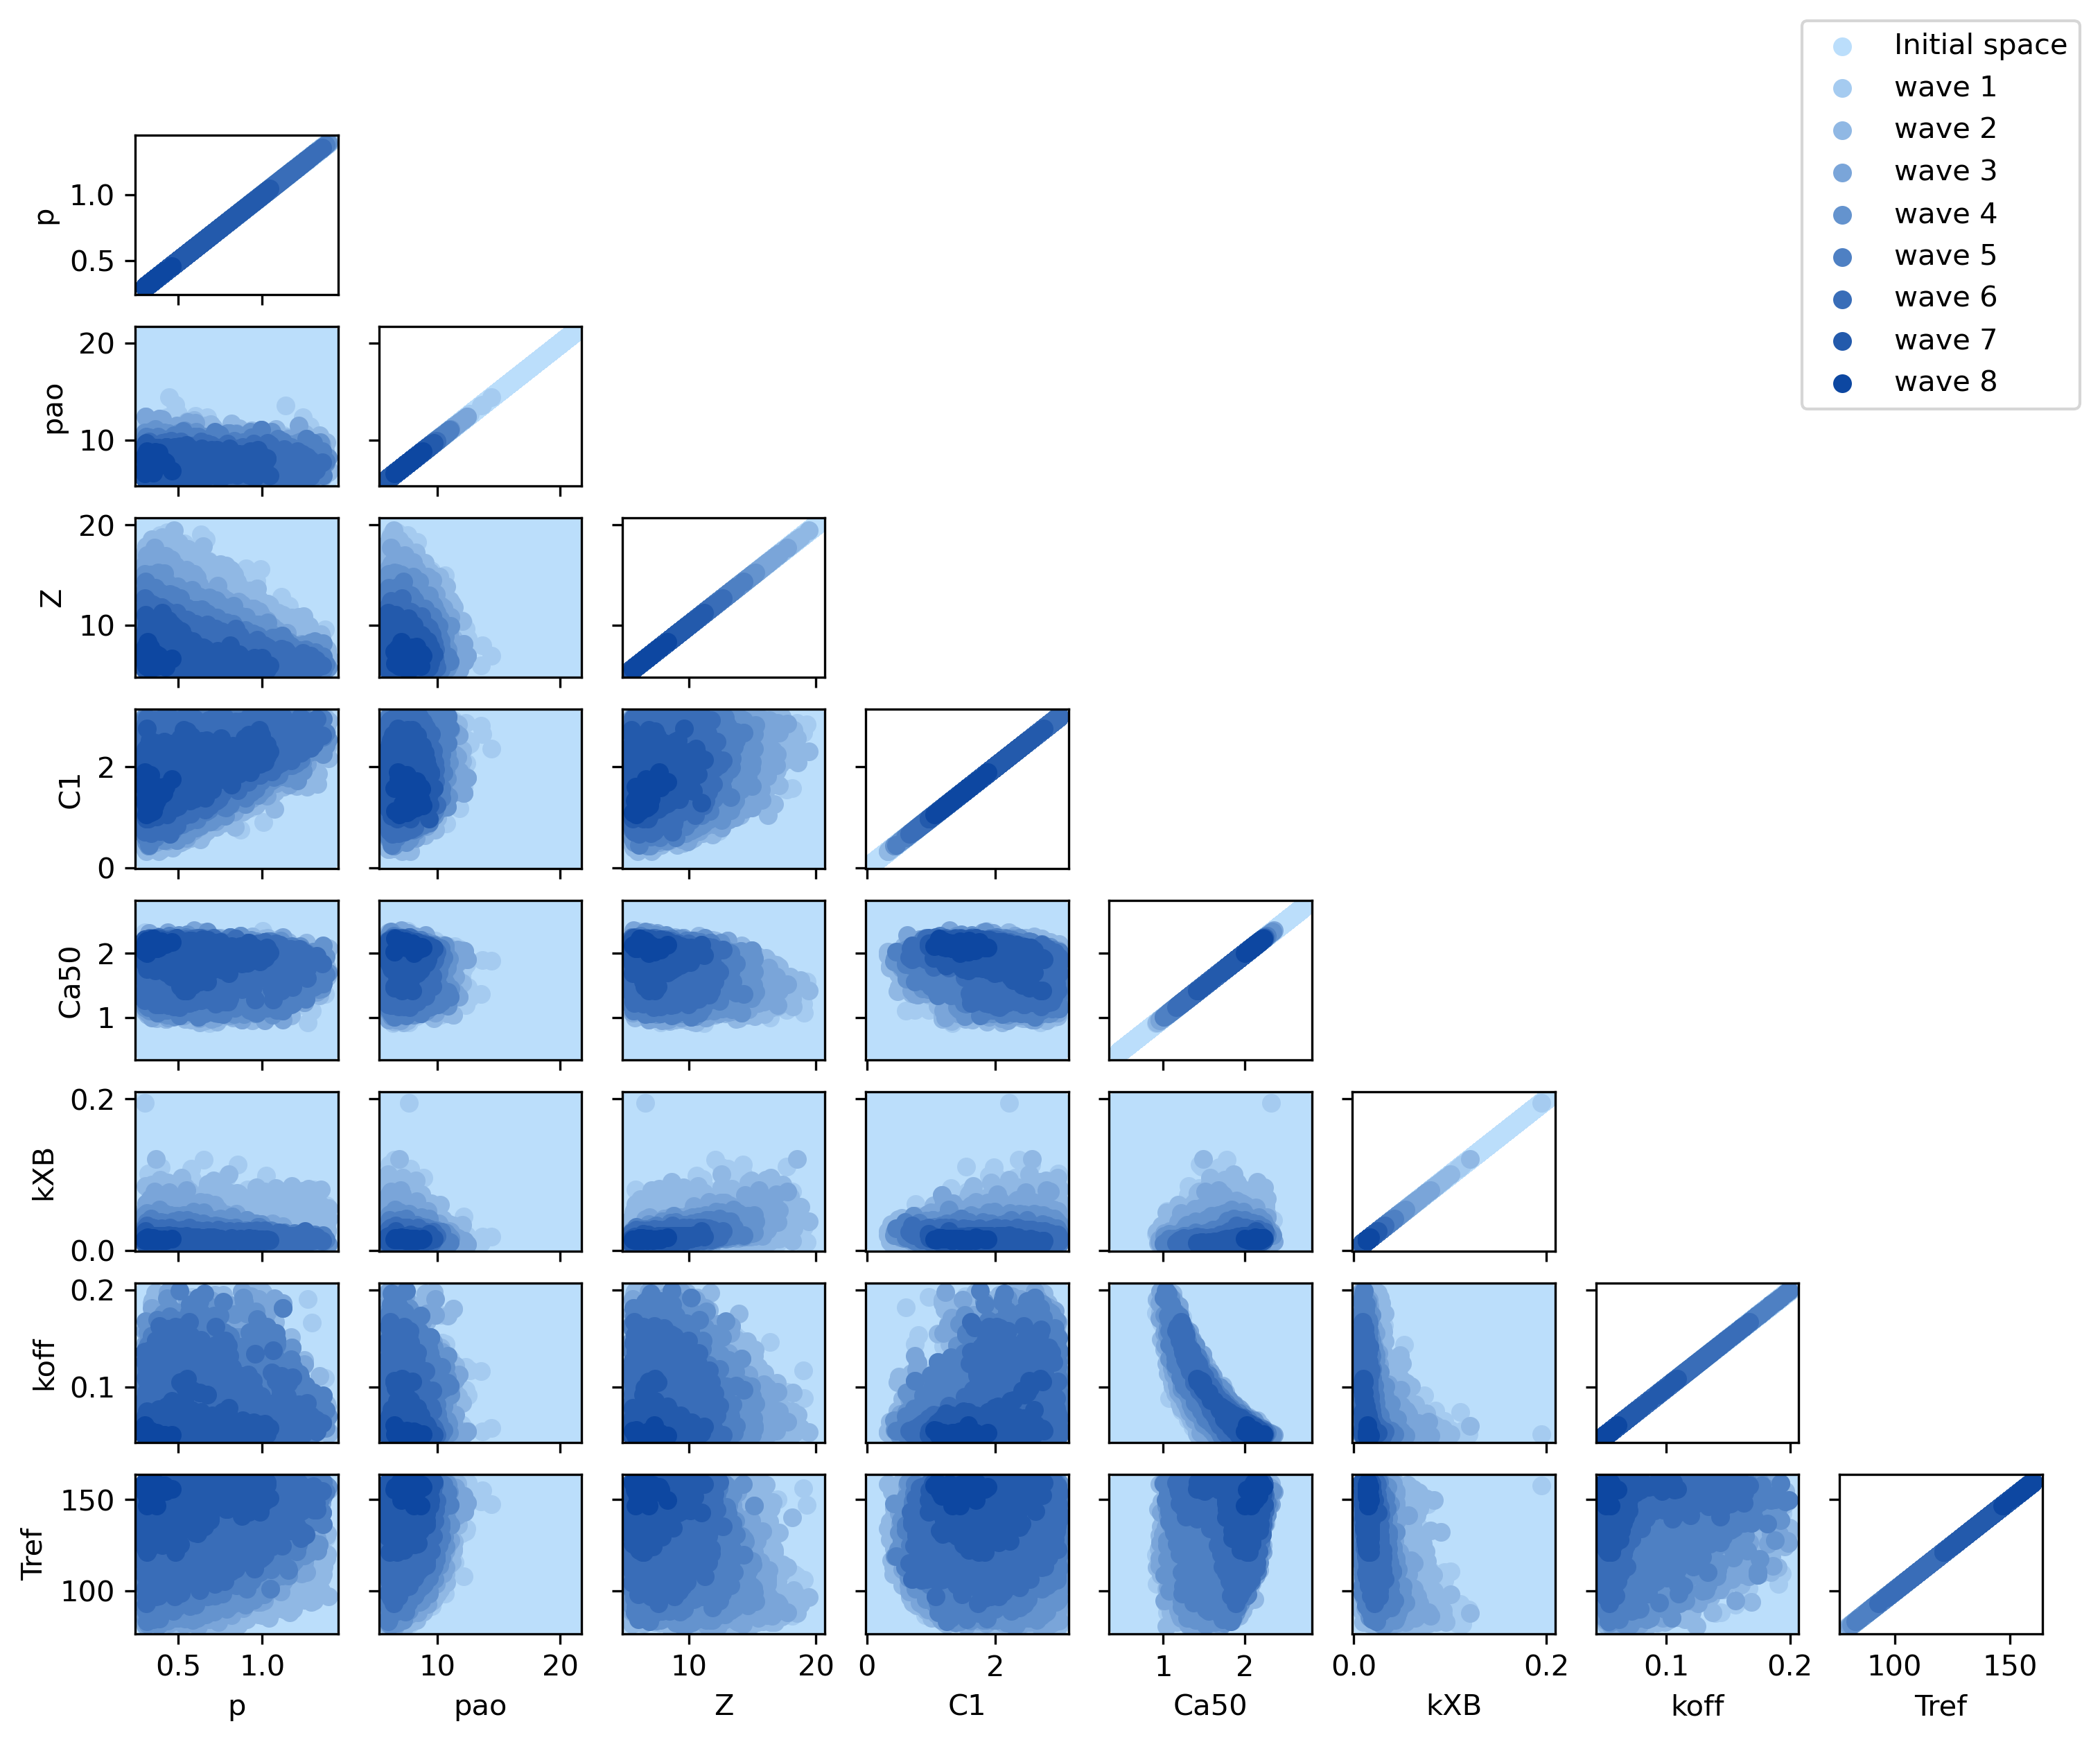
\includegraphics[width=\textwidth]{figures/chapter04/hm_sham.png}
    \caption{High-dimensional input parameter space reduction during SHAM history matching. SHAM HM completed within eight waves.}
    \label{fig:shamhm}
\end{figure}

\begin{figure}[!ht]
    \myfloatalign
    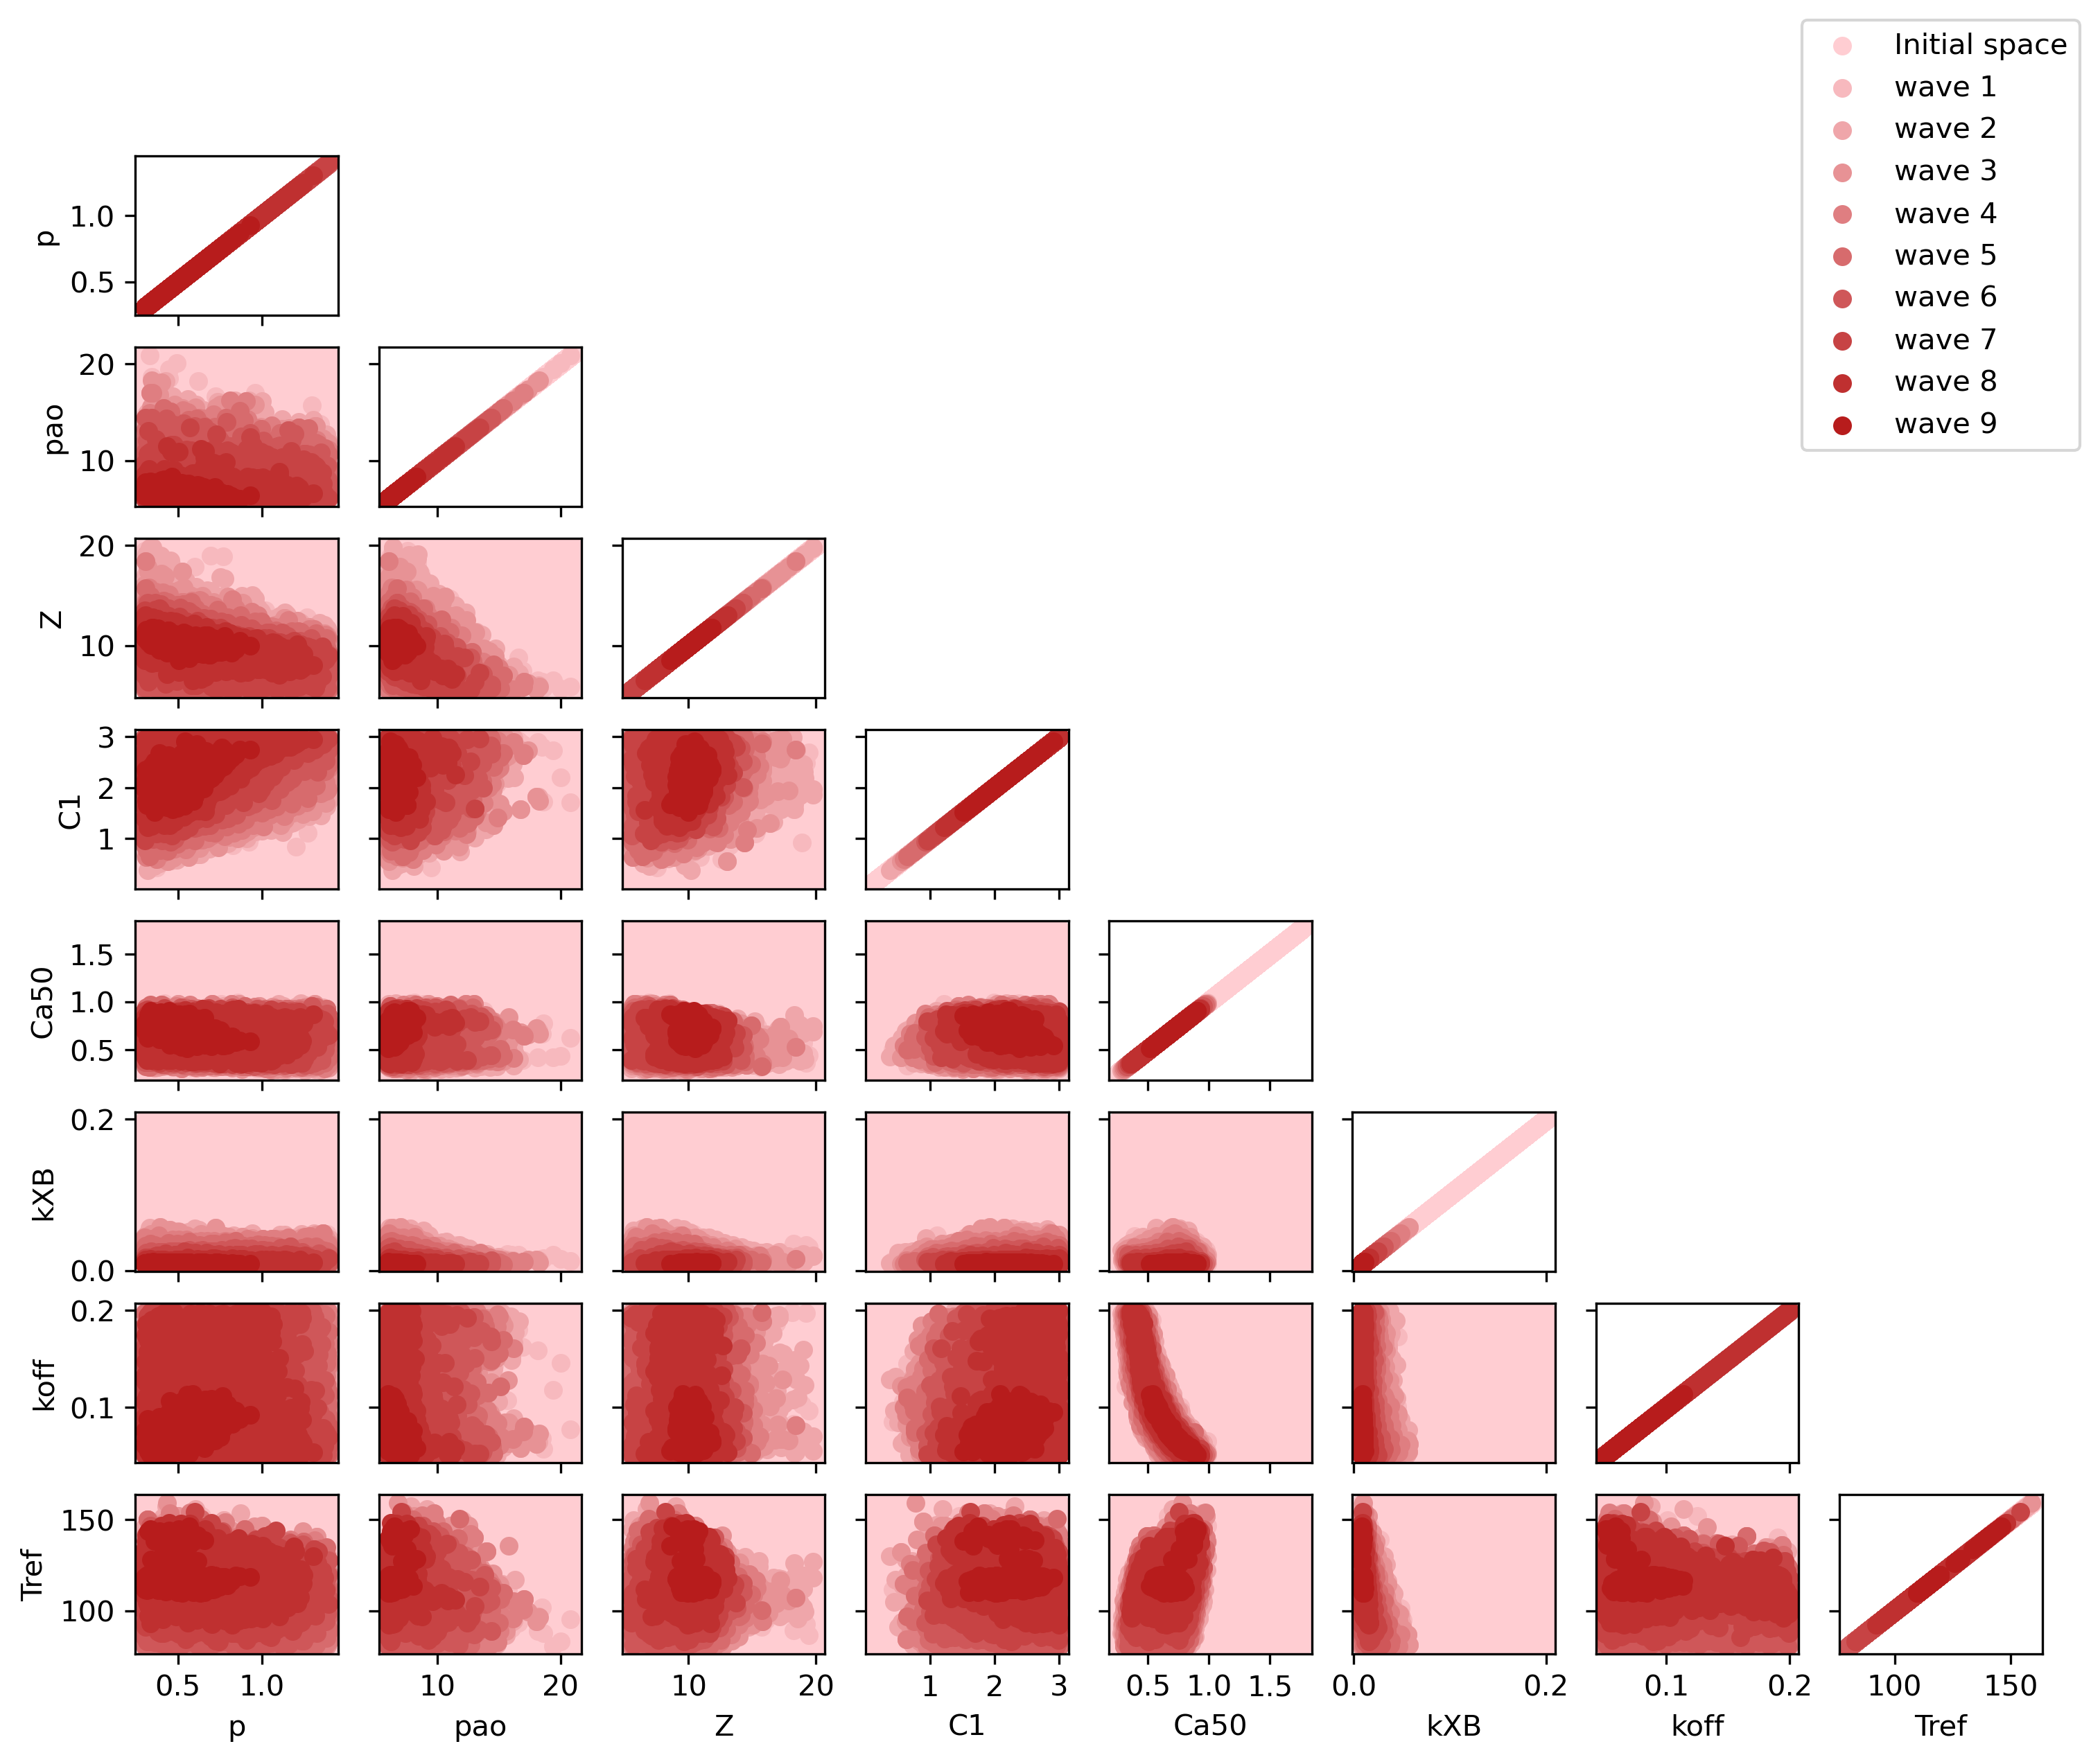
\includegraphics[width=\textwidth]{figures/chapter04/hm_ab.png}
    \caption{High-dimensional input parameter space reduction during AB history matching. AB HM completed within nine waves.}
    \label{fig:abhm}
\end{figure}

\begin{table}[!ht]
    \myfloatalign
    \begin{tabularx}{\textwidth}{lXXXX}
        \toprule
        \tableheadline{Wave} & \multicolumn{4}{c}{\spacedlowsmallcaps{Rat}} \\
        \midrule
        & \multicolumn{2}{c}{\spacedlowsmallcaps{SHAM}} & \multicolumn{2}{c}{\spacedlowsmallcaps{AB}} \\
        \midrule
        & $I_{\,\text{cutoff}}$ & NIMP ($\SI{}{\percent}$) & $I_{\,\text{cutoff}}$ & NIMP ($\SI{}{\percent}$) \\
        \midrule
        $1$ & $5.5$ & $ 0.09$ & $5.0$ & $ 0.08$ \\
        $2$ & $5.0$ & $41.79$ & $4.5$ & $65.66$ \\
        $3$ & $4.5$ & $25.63$ & $4.0$ & $59.89$ \\
        $4$ & $4.0$ & $49.47$ & $3.5$ & $61.29$ \\
        $5$ & $3.5$ & $28.22$ & $3.0$ & $43.46$ \\
        $6$ & $3.0$ & $12.05$ & $3.0$ & $30.59$ \\
        $7$ & $3.0$ & $ 8.56$ & $3.0$ & $21.33$ \\
        $8$ & $3.0$ & $ 0.09$ & $3.0$ & $12.93$ \\
        $9$ & $-$   & $-$     & $3.0$ & $ 1.15$ \\
        \bottomrule
    \end{tabularx}
    \caption{Details of history matching progression for the SHAM and AB rat models' fitting. At each wave, parameter points are tested against an implausibility criterion using the reported cutoff values ($I_{\,\text{cutoff}}$), and only a percentage of these points (NIMP) out of the total tested points resulted to be non-implausible.}
    \label{tab:hmdetails}
\end{table}

\vspace{0.2cm}
Although HM does not ensure the reduction in individual parameters' ranges but rather a whole high-dimensional space reduction \cite{Coveney:2018}, the diagonal plots in Figures~\ref{fig:shamhm}--\ref{fig:abhm} suggest that all the parameters underwent reduction (to different degrees) along their $1$D domain, both in the SHAM and AB models. We therefore analysed whether these parameters had been constrained to lie in spaces which differ according to the rat phenotype. This phenomenon was observed in $5$ of the $8$ total parameters, as highlighted in Figure~\ref{fig:onedspacered}. We can see that $z$, $\Caif$, $\kxb$, $\koff$ and $\tref$ take values in completely separated spaces for the SHAM and AB models. The biggest space separation is observed for $\Caif$ and $\tref$.

\begin{figure}[!ht]
    \myfloatalign
    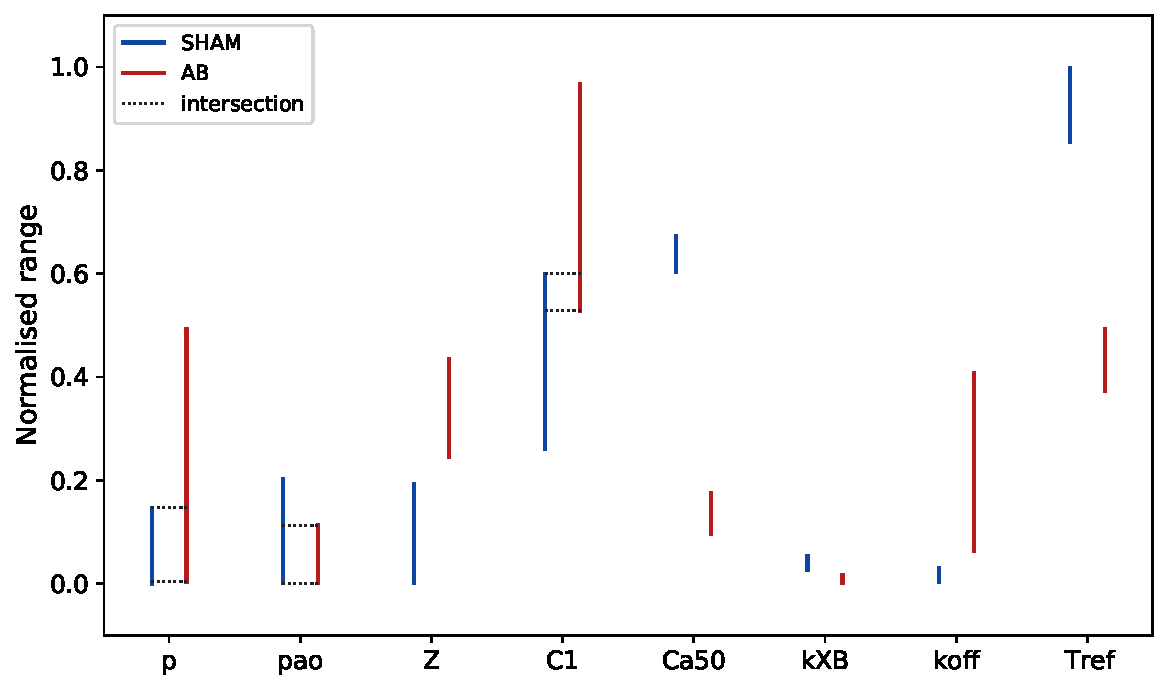
\includegraphics[width=0.8\textwidth]{figures/chapter04/sham_vs_ab_final_ranges.pdf}
    \caption{Input parameters’ one-dimensional ranges after completing HM procedure. Comparison between SHAM (blue) and AB (red) rat models’ fittings. For each input parameter, the displayed intervals are scaled according to the initial range for that specific parameter. When SHAM and AB intervals’ intersection is non-empty, this is also displayed with dotted lines.}
    \label{fig:onedspacered}
\end{figure}


%
%
%
\subsection{Fitted models}\label{sec:ch4fittedmodels}
We finally investigated whether the constrained input parameter space was mapped by the simulator into model read-outs that matched experimental observations. For this purpose, we sampled using the cloud technique and simulated $1,024$ points in the HM final wave's $X_{NIMP}$ parameter space of both the SHAM and AB models. Of these, only $264$ and $178$ points led to a successfully completed simulation for SHAM and AB models, respectively. After extracting the LV features from the simulator outputs, we examined their distributions and compared them to the same features' experimentally observed variability (Table~\ref{tab:values2match}). This is summarised in Figure~\ref{fig:simulatormatchtoexpvar}.

\begin{figure}[!ht]
    \myfloatalign
    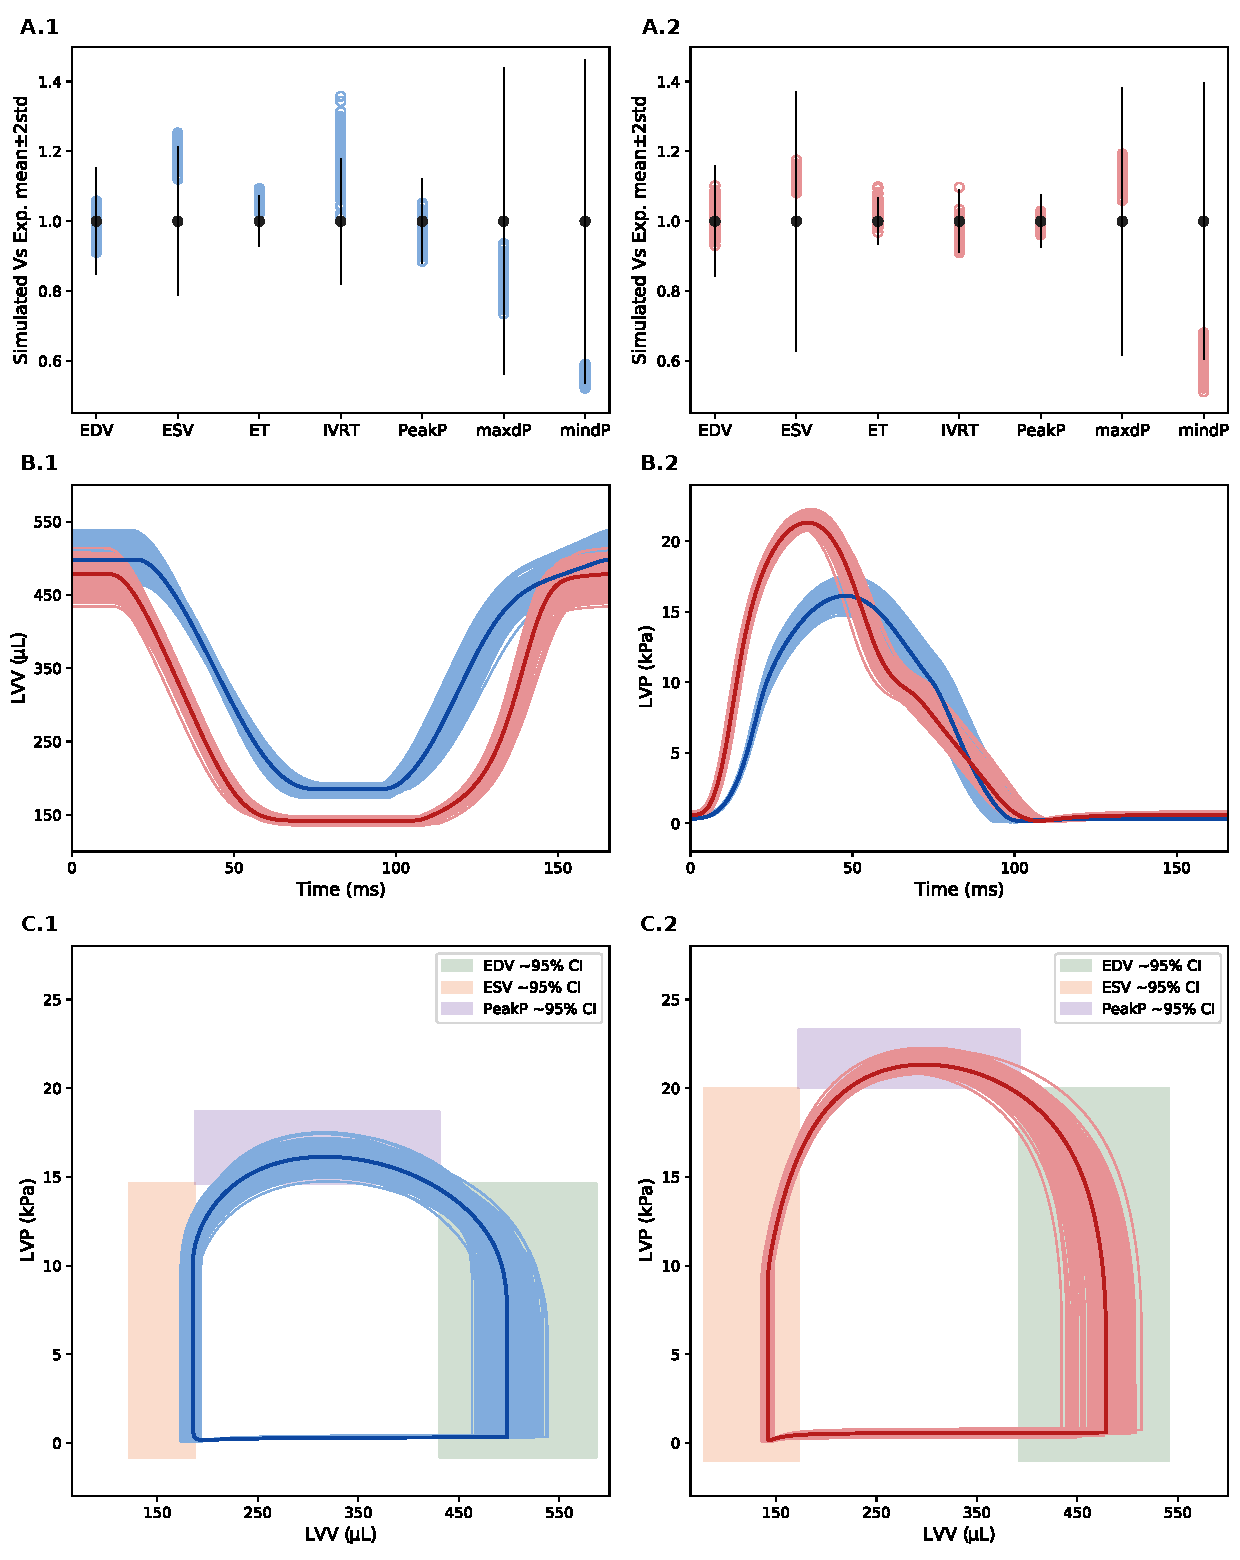
\includegraphics[width=\textwidth]{figures/chapter04/sham_vs_ab_fit.pdf}
    \caption{Simulator runs using the HM last wave’s $X_{NIMP}$ points as an input. (A) Obtained LV features’ (empty, coloured dots) distributions around experimental mean values (filled, black dots) for SHAM (.$1$) and AB (.$2$). $2$ standard deviations confidence intervals are shown as vertical straight lines centred in their respective mean value. All the displayed values (including confidence intervals) are normalized by the respective experimental mean values. (B) Simulated LV volume (.$1$) and pressure (.$2$) curves which the features in (A) were extracted from, for SHAM (blue) and AB (red). The average curves are displayed in darker colour variant. (C) Resulting SHAM (.$1$) and AB (.$2$) pressure-volume loops with approximately $\SI{95}{\percent}$ EDV, ESV, PeakP features’ experimental confidence intervals. \todo{add A-B-C tags}}
    \label{fig:simulatormatchtoexpvar}
\end{figure}

\vspace{0.2cm}\noindent
Figures~\ref{fig:simulatormatchtoexpvar}A.$1$--$2$ show that points belonging to the reduced input parameter space reproduce the majority of the emerging organ-scale LV features except $\textrm{ESV}$, $\textrm{maxdP}$ and $\textrm{mindP}$ which distribute far from the experimentally observed mean values. The simulated LV volume and pressure transients which the features were extracted from are also reported (Figures~\ref{fig:simulatormatchtoexpvar}B.$1$--$2$). The resulting pressure-volume loops are provided in Figures~\ref{fig:simulatormatchtoexpvar}C.$1$--$2$.
By comparing the highlighted average curves, we can notice smaller end-diastolic and end-systolic volumes for AB, which in turn still preserve the ejection fraction observed in the control. Diastolic time is increased in AB due to an increase in IVRT. LV peak pressure is visibly higher in AB.

\vspace{0.2cm}
\todo{Talk about best fit rep models}

\begin{table}[!ht]
    \myfloatalign
    \begin{tabular}{@{}llll}
    \toprule
    \tableheadline{Parameter} & \tableheadline{Units}                        & \multicolumn{2}{c}{\spacedlowsmallcaps{Value}} \\ \midrule
                       &                                       & \tableheadline{SHAM} & \tableheadline{ZSF1} \\ \midrule
    $\dca$     & $\SI{}{\micro\Molar}$                 & $0.4632$      & $0.5870$ \\
    $\ampl$    & $\SI{}{\micro\Molar}$                 & $1.0341$      & $1.0317$ \\
    $\tp$      & $\SI{}{\milli\second}$                & $25.9474$     & $25.9474$ \\
    $\rtf$    & $\SI{}{\milli\second}$                & $40.0807$     & $40.0807$ \\
    $\Caif$            & $\SI{}{\micro\Molar\tothe{1-1/\ntrpn}}$                 & $2.1723$      & $2.1723$ \\
    $\beta_1$          & $-$                             & $-1.5$        & $-1.5$ \\
    $\koff$            & $\SI{}{\per\milli\second}$            & $0.0515$      & $0.0515$ \\
    $\ntrpn$           & $-$                             & $2.0$         & $2.0$ \\
    $\kxb$             & $\SI{}{\per\milli\second}$            & $0.0172$      & $0.0172$ \\
    $\nxb$             & $-$                             & $5.0$         & $5.0$ \\
    $\trpnf$           & $-$                             & $0.35$        & $0.35$ \\
    $\tref$            & $\SI{}{\kilo\pascal}$                 & $156.067$     & $156.067$ \\
    $p$                & $\SI{}{\kilo\pascal}$                 & $0.3122$      & $0.4481$ \\
    $\pao$             & $\SI{}{\kilo\pascal}$                 & $7.1136$      & $10.3887$ \\
    $Z$                & $\SI{}{\mmHg\second\per\milli\liter}$ & $5.6234$      & $7.4031$ \\
    $C_1$              & $\SI{}{\kilo\pascal}$                          & $0.9141$      & $1.0670$ \\
    \bottomrule
    \end{tabular}
    \caption{Representative SHAM rat and ZSF1 rat models input parameters' values.}
    \label{tab:shamabbestfitparameters}
\end{table}

\begin{table}[!ht]
    \myfloatalign
    \begin{tabular}{@{}llll}
    \toprule
    \tableheadline{LV feature}             & \tableheadline{Units}                         & \multicolumn{2}{c}{\spacedlowsmallcaps{Value}} \\ \midrule
                                    &                                        & \tableheadline{SHAM} & \tableheadline{ZSF1} \\ \midrule
    $\textrm{EDV}$                  & $\SI{}{\micro\liter}$                  & $516.23$      & $444.02$ \\
    $\textrm{ESV}$                  & $\SI{}{\micro\liter}$                  & $173.82$      & $172.83$ \\
    $\textrm{EF}$                   & $\SI{}{\percent}$                      & $66.33$       & $61.08$ \\
    $\textrm{IVCT}$                 & $\SI{}{\milli\second}$                 & $19.3$        & $19.7$ \\
    $\textrm{ET}$                   & $\SI{}{\milli\second}$                 & $52.9$        & $54.6$ \\
    $\textrm{IVRT}$                 & $\SI{}{\milli\second}$                 & $23.8$        & $33.0$ \\
    $\textrm{Tdiast}$               & $\SI{}{\milli\second}$                 & $93.5$        & $91.4$ \\
    $\textrm{PeakP}$                & $\SI{}{\kilo\pascal}$                  & $16.15$       & $19.15$ \\
    $\textrm{Tpeak}$                & $\SI{}{\milli\second}$                 & $46.6$        & $45.9$ \\
    $\textrm{ESP}$                  & $\SI{}{\kilo\pascal}$                  & $10.04$       & $12.55$ \\
    $\textrm{maxdP}$ & $\SI{}{\kilo\pascal\per\milli\second}$ & $0.9973$      & $1.1700$ \\
    $\textrm{mindP}$ & $\SI{}{\kilo\pascal\per\milli\second}$ & $-0.5712$     & $-0.5276$ \\
    \bottomrule
    \end{tabular}
    \caption{Representative SHAM rat and ZSF1 rat models output LV features' values.}
    \label{tab:shamabbestfitfeatures}
\end{table}


%
%
%
\section{Discussion}\label{sec:ch4discussion}
\todo{this is Discussion copy-pasted from the paper: adapt it to thesis}

\noindent
In this study, we have shown how GPEs can be used to rapidly and robustly tune a multi-scale rat heart model to organ-scale functional measurements and characterise the global sensitivity of the model. This is the first example, to the best of our knowledge, of the use of HM to constrain multi-scale cardiac mechanics models. Previous attempts to tune cardiac mechanics model parameters have sequentially fitted parameters \cite{Wang:2009} or fitted a maximum of $2$--$4$ parameters using deterministic approaches \cite{Lewalle:2018}. Here we fitted $8$ parameters concurrently. This means that error is evenly distributed across parameters and does not accumulate in the latter parameters as occurs in sequential fitting. We showed that active and passive parameters can be fitted simultaneously, avoiding potential confounding effects of slow relaxation, as occurs in heart failure models \cite{Xi:2013}. In addition, by providing bounds on model parameters (therefore an estimate of parameter uncertainty), the HM technique is compatible with verification, validation and uncertainty quantification (VVUQ) methods \cite{Patten:2009} supported by the ASME V$\&$V40 standards and the FDA \cite{Asme:2019}.

HM produced different constraints for the SHAM and AB models, even if starting from the same hypercube in the input parameter space. Interestingly, the separation across the two rat phenotypes in the $1$D parameters' ranges occurs mostly for parameters describing active tension development at the cellular level. We interpret this result as a confirmation that impaired whole-organ function in the AB rat is linked to altered properties at the cell level.

We have performed the first GSA of cardiac mechanics. Previous models have performed local sensitivity analysis \cite{Sher:2013}, or attempted GSA on simplified cardiac cell models \cite{Pathmanathan:2019}. Our GSA approach highlighted that left ventricular function is mostly influenced by cellular-level properties, consistent with our HM results.

\vspace{0.2cm}\noindent
\todo{this is Limitations copy-pasted from the paper: adapt it to thesis}

\noindent
We have developed a detailed biophysical rat heart model. However, this model is inherently a simplification of the underlying system, with four specific limitations.

Firstly, the boundary conditions do not account for the pericardium that may be important in constraining cardiac mechanics \cite{Strocchi:2020}. We have not accounted for potential spatial variations in cellular properties and $\textrm{Ca}^{2+}$ transients, and the latter homogeneously activates contraction throughout ventricular walls. Extending the sensitivity analysis to include $\textrm{Ca}^{2+}$ transient features would allow us to estimate if this has a major effect on our results.

Secondly, HM provides a bounded region of non-implausible parameter sets. Parameter bounds do not define parameter distributions. Including a MCMC parameter fit using the HM bounds as priors would extend this method to estimate likely parameter distributions as opposed to parameter bounds.

The heterogeneity of the data used to constrain the models is another limitation. Specifically, pressure measurements were not available for the rats used as an animal model and were therefore collected and averaged over similar experimental studies. Related to this, we only used a single representative anatomy for the healthy rats' cohort and single representative anatomy for the aortic-banded rats' cohort: ejection time and isovolumetric relaxation time features were constrained according to single measurements coming from these two anatomies' segmentations.

The fourth limitation concerns the GPE, HM and GSA implementations. In Section we have fitted the mean function separately and then trained the GP on the residuals, following the GPE-HM approach applied previously~\cite{Salter:2016,Vernon:2018}. However, different emulation strategies exist (see e.g.)~\cite{Oakley:2004}, where the linear regression model parameters and the GP hyperparameters are jointly optimised;~\cite{Coveney:2018} uses this GP formulation for HM), and may impact the implausibility measure. To test if this choice of GP formulation impacted our final results we have preformed a preliminary comparison with the Oakley and O'Hagan~\cite{Oakley:2004} emulation strategy (see Supplementary materials). This suggests that HM can potentially converge to the same reduced parameter space, however, the optimal choice of GP for fitting cardiac models requires further research.

For both HM and GSA we used independent GPEs for each output. This univariate approach provided us the flexibility to tune the hyperparameters and choose basis functions for each output independently. However, it did not account for potential correlations in outputs, which could be accounted for with a multi-output strategy e.g.~\cite{Conti:2009}, although this assumes common hyperparameters across all outputs. A multi-variate implausibility measure could be constructed from multi-output GPEs, which could potentially assist in ruling out more implausible parameter space.

In the implausibility measure (equation ($4$) in the Supplementary materials) calculation we omitted the model discrepancy term, for which we did not have any estimate available. To completely replace animal models with virtual representations of them, further experts knowledge will be needed to quantify the difference between the \textit{in-silico} model and the real world system that it represents. 

Finally, global sensitivity indices were estimated using the mean of the available emulator, ignoring the uncertainty of the emulator itself. However, the emulator's uncertainty was small, therefore the estimated sensitivity indices were still able to capture the parameters' influence on the model outputs (see Supplementary materials for an example on ejection fraction feature). This can be further improved in future studies by looking for alternative estimations of the sensitivity indices which directly make use of the emulator mean and variance.

\vspace{0.2cm}\noindent
\todo{this is Conclusion copy-pasted from the paper: adapt it to thesis}

\noindent
We have shown that GPE can effectively be used to robustly and rapidly constrain multi-scale cardiac models from organ-scale measurements. The obtained virtual bi-ventricular rat hearts are a valuable system to be used for further investigation of heart failure. Moreover, we demonstrated that our GPE-based GSA approach enables the computationally efficient identification of key components in 3D ventricular mechanics, giving a deeper insight into the link between cell, tissue, shape and boundary conditions properties and organ-scale function.